\section{Chillers }\label{chillers}

\subsection{Absorption Chiller}\label{absorption-chiller}

The input object Chiller:Absorption provides a model for absorption chillers that is an empirical model of a standard absorption refrigeration cycle.~ The condenser and evaporator are similar to that of a standard chiller, which are both water-to-water heat exchangers.~ The assembly of a generator and absorber provides the compression operation.~ Low-pressure vapor from the evaporator is absorbed by the liquid solution in the absorber.~ A pump receives low-pressure liquid from the absorber, elevates the pressure of the liquid, and delivers the liquid to the generator.~ In the generator, heat from a high temperature source (hot water or steam) drives off the vapor that has been absorbed by the solution.~ The liquid solution returns to the absorber through a throttling valve whose purpose is to provide a pressure drop to maintain the pressure difference between the generator and absorber.~ The heat supplied to the absorber can be waste heat from a diesel jacket, or the exhaust heat from diesel, gas, and steam turbines.~ For more information on absorption chillers, see the Input/Output Reference Document (Object: Chiller:Absorption).

The part-load ratio of the absoprtion chiller's evaporator is simply the actual cooling effect produced by the chiller divided by the maximum cooling effect available.

\begin{equation}
PLR = \frac{\dot{Q}_{evap}}{\dot{Q}_{evap,rated}}
\end{equation}

where:

\(PLR\) is the part-load ratio of chiller evaporator

\({\dot Q_{evap}}\) is the chiller evaporator load {[}W{]}

\({\dot Q_{evap,\,rated}}\) is the rated chiller evaporator capacity {[}W{]}.

This absorption chiller model is based on a polynomial fit of absorber performance data.~ The Generator Heat Input Part Load Ratio Curve is a quadratic equation that determines the ratio of the generator heat input to the \emph{demand} on the chiller's evaporator (Q\(_{evap}\)).

\begin{equation}
GeneratorHeatInputRatio = \frac{{C1}}{{PLR}} + C2 + C3\left( {PLR} \right)
\end{equation}

The Pump Electric Use Part Load Ratio Curve is a quadratic equation that determines the ratio of the actual absorber pumping power to the nominal pumping power.

\begin{equation}
ElectricInputRatio = C1 + C2 * PLR + C3 * PL{R^2}
\end{equation}

Thus, the coefficient sets establish the ratio of heat power in-to-cooling effect produced as a function of part load ratio.~ The ratio of heat-power-in to cooling-effect-produced is the inverse of the coefficient of performance.

If the operating part-load ratio is greater than the minimum part-load ratio, the chiller will run the entire time step and cycling will not occur (i.e. \emph{CyclingFrac} = 1). If the operating part-load ratio is less than the minimum part-load ratio, the chiller will be on for a fraction of the time step equal to \emph{CyclingFrac}. Steam (or hot water) and pump electrical energy use are also calculated using the chiller part-load cycling fraction.

\begin{equation}
CyclingFrac = MIN\left( {1,\frac{{PLR}}{{PL{R_{min}}}}} \right)
\end{equation}

\begin{equation}
{\dot Q_{generator}} = GeneratorHeatInputRatio\left( {{{\dot Q}_{evap}}} \right)\left( {CyclingFrac} \right)
\end{equation}

\begin{equation}
{\dot Q_{pump}} = ElectricInputRatio\left( {{P_{pump}}} \right)\left( {CyclingFrac} \right)
\end{equation}

where:

\(CyclingFrac\) is the chiller part-load cycling fraction

\(PL{R_{min}}\) is the chiller minimum part-load ratio

\({\dot Q_{generator}}\) is the generator input power (W)

\({\dot Q_{pump}}\) is the absorbtion chiller pumping power (W).

The evaporator water mass flow rate is calculated based on the Chiller Flow Mode as follows.

\textbf{Constant Flow Chillers:}

\begin{equation}
{\dot m_{evap}} = {\dot m_{evap,max}}
\end{equation}

\textbf{Variable Flow Chillers:}

\begin{equation}
\Delta {T_{evap}} = {T_{evap,\,in}} - {T_{evap,\,SP}}
\end{equation}

\begin{equation}
  \dot{m}_{evap} = \frac{\dot{Q}_{evap}}{C_{p,evap} \Delta T_{evap}}
\end{equation}

where:

\({\dot m_{evap}}\) is the chiller evaporator water mass flow rate (kg/s)

\({\dot m_{evap,\,max}}\) is the chiller design evaporator water mass flow rate (kg/s)

\(\Delta {T_{evap}}\) is the chiller evaporator water temperature difference (\(^{\circ}\)C)

\({T_{evap,\,in}}\) is the chiller evaporator inlet water temperature (\(^{\circ}\)C)

\({T_{evap,\,SP}}\) is the chiller evaporator outlet water setpoint temperature (\(^{\circ}\)C)

\({C_p}\) is the = specific heat of water entering evaporator (J/kg-\(^{\circ}\)C).

The evaporator outlet water temperature is then calculated based on the cooling effect produced and the evaporator entering water temperature.

\begin{equation}
  T_{evap,out} = T_{evap,in} + \frac{\dot{Q}_{evap}}{\dot{m}_{evap}C_{p,evap}}
\end{equation}

where:

\({T_{evap,out}}\) is the chiller evaporator outlet water temperature (\(^{\circ}\)C)

\({T_{evap,in}}\) is the chiller evaporator inlet water temperature (\(^{\circ}\)C)

\({C_{p,\,evap}}\) is the specific heat of chiller evaporator inlet water (J/kg-\(^{\circ}\)C)

\({\dot m_{evap}}\) is the chiller evaporator water mass flow rate (kg/s).

The condenser heat transfer and condenser leaving water temperature are also calculated.

\begin{equation}
{\dot Q_{cond}} = {\dot Q_{evap}} + {\dot Q_{generator}} + {\dot Q_{pump}}
\end{equation}

\begin{equation}
  T_{cond,out} = T_{cond,in} + \frac{\dot{Q}_{cond}}{\dot{m}_{cond}C_{p,cond}}
\end{equation}

where:

\({\dot Q_{cond}}\) is the chiller condenser heat transfer rate (W)

\({T_{cond,out}}\) is the chiller condenser outlet water temperature (\(^{\circ}\)C)

\({T_{cond,in}}\) is the chiller condenser inlet water temperature (\(^{\circ}\)C)

\({C_{p,\,cond}}\) is the specific heat of chiller condenser inlet water (J/kg-\(^{\circ}\)C)

\({\dot m_{cond}}\) is the chiller condenser water mass flow rate (kg/s).

The absorption chiller can model the impact of steam or hot water entering the generator, although the connection of the steam (hot water) nodes to a plant is not actually required. The calculations specific to the generator depend on the type of fluid used and are described here in further detail.

\subsubsection{Steam Loop Calculations}\label{steam-loop-calculations}

When a steam loop is used and the inlet and outlet node names are specified (i.e.~the nodes are connected to a steam loop), the generator outlet node steam mass flow rate and temperature are calculated based on the generator input power, latent heat of steam, the specific heat of water, and the amount of subcooling in the steam generator. The model assumes dry saturated steam enters the absorption chiller's generator and exits the generator as a subcooled liquid. The temperature leaving the generator is calculated based on the user entered amount of liquid subcooling in the generator. The effect of subcooling of the liquid (condensate) in the pipe returning to the boiler is not modeled.

\begin{equation}
{\dot m_{steam}}\,\,\,\, = \,\,\,\,\,\frac{{{{\dot Q}_{generator}}}}{{{h_{fg}} + {c_{p,\,water}} \times \Delta {T_{sc}}}}
\end{equation}

\begin{equation}
{T_{generator,out}} = {T_{generator,in}} - \Delta {T_{sc}}
\end{equation}

where:

\({\dot m_{steam}}\) is the chiller steam mass flow rate (kg/s)

\({h_{fg}}\) is the latent heat of steam (J/kg)

\({c_{p,\,water}}\) is the specific heat of saturated water in the generator (J/kg-\(^{\circ}\)C)

\(\Delta {T_{sc}}\) is the amount of subcooling in steam generator (\(^{\circ}\)C)

\({T_{generator,out}}\) is the generator steam outlet node temperature (\(^{\circ}\)C)

\({T_{generator,in}}\) is the generator steam inlet node temperature (\(^{\circ}\)C).

\subsubsection{Hot Water Loop Calculations}\label{hot-water-loop-calculations}

When a hot water loop is used and the inlet and outlet node names are specified (i.e.~the nodes are connected to a hot water loop), the generator outlet node temperature is calculated based on the generator input power, mass flow rate of water, and the specific heat of water entering the hot water generator. The calculations are based on the Chiller Flow Mode as follows.

\textbf{Constant Flow Chillers:}

\begin{equation}
{\dot m_{generator}} = {\dot m_{generator,max}}
\end{equation}

\textbf{Variable Flow Chillers:}

\begin{equation}
  \dot{m}_{generator} = \frac{\dot{Q}_{generator}}{C_{p,water}\Delta T_{generator}}
\end{equation}

\begin{equation}
{T_{generator,out}} = {T_{generator,in}} - \frac{{{{\dot Q}_{generator}}}}{{{{\dot m}_{generator}}\left( {{C_{p\,,\,water}}} \right)}}
\end{equation}

where:

\({\dot m_{generator}}\) is the generator hot water mass flow rate (kg/s)

\({\dot m_{generator,\,max}}\) is the generator design hot water mass flow rate (kg/s)

\(\Delta {T_{generator}}\) is the generator design hot water temperature difference (\(^{\circ}\)C).

\subsection{Indirect Absorption Chiller}\label{indirect-absorption-chiller}

The Chiller:Absorption:Indirect object is an enhanced version of the absorption chiller model found in the Building Loads and System Thermodynamics (BLAST) program. This enhanced model is nearly identical to the existing absorption chiller model (Ref. Chiller:Absorption) with the exceptions that: 1) the enhanced indirect absorption chiller model provides more flexible performance curves and 2) chiller performance now includes the impact of varying evaporator, condenser, and generator temperatures. Since these absorption chiller models are nearly identical (i.e., the performance curves of the enhanced model can be manipulated to produce similar results to the previous model), it is quite probable that the Chiller:Absorption model will be deprecated in a future release of EnergyPlus.

The indirect absorption chiller's condenser and evaporator are similar to that of a standard chiller, which are both water-to-water heat exchangers. The assembly of a generator and absorber provides the compression operation. A schematic of a single-stage absorption chiller is shown in the figure below. Low-pressure vapor from the evaporator is absorbed by the liquid solution in the absorber. A pump receives low-pressure liquid from the absorber, elevates the pressure of the liquid, and delivers the liquid to the generator. In the generator, heat from a high temperature source (hot water or steam) drives off the vapor that has been absorbed by the solution. The liquid solution returns to the absorber through a throttling valve whose purpose is to provide a pressure drop to maintain the pressure difference between the generator and absorber. The heat supplied to the generator can be either hot water or steam, however, connection to an actual plant loop is not required. For more information on indirect absorption chillers, see the Input/Output Reference Document (Object: Chiller:Absorption:Indirect).

\begin{figure}[hbtp] % fig 160
\centering

\includegraphics[width=0.9\textwidth, height=0.9\textheight, keepaspectratio=true]{media/image3060.png}
\caption{Schematic Diagram of a Single-Stage Absorption Chiller \protect \label{fig:schematic-diagram-of-a-single-stage}}
\end{figure}

The chiller cooling effect (capacity) will change with a change in condenser water temperature. Similarly, the chiller cooling effect will change as the temperature of the evaporator water changes. The chiller cooling effect will also change with a change in or generator inlet water temperature and only applies when Hot Water is used as the generator heat source. A quadratic or cubic equation is used to modify the rated chiller capacity as a function of both the condenser and generator inlet water temperatures and the evaporator outlet water temperature. If any or all of the capacity correction factor curves are not used, the correction factors are assumed to be 1.

\begin{equation}
CAPF{T_{evaporator}} = a + b\left( {{T_{evaporator}}} \right) + c{\left( {{T_{evaporator}}} \right)^2} + d{\left( {{T_{evaporator}}} \right)^3}
\end{equation}

\begin{equation}
CAPF{T_{condenser}} = e + f\left( {{T_{condenser}}} \right) + g{\left( {{T_{condenser}}} \right)^2} + h{\left( {{T_{condenser}}} \right)^3}
\end{equation}

\(CAPF{T_{generator}} = i + j\left( {{T_{generator}}} \right) + k{\left( {{T_{generator}}} \right)^2} + l{\left( {{T_{generator}}} \right)^3}\) ~(\emph{Hot Water only})

\begin{equation}
{\dot{Q}_{evap,max}} = {\dot{Q}_{evap,rated}}\left( {CAPF{T_{evaporator}}} \right)\left( {CAPF{T_{condenser}}} \right)\left( {CAPF{T_{generator}}} \right)
\end{equation}

where:

\(CAPF{T_{evaporator}}\) is the capacity correction (function of evaporator temperature) factor

\(CAPF{T_{condenser}}\) is the capacity correction (function of condenser temperature) factor

\(CAPF{T_{generator}}\) is the capacity correction (function of generator temperature) factor

\({T_{evaporator}}\) is the evaporator outet water temperature (\(^{\circ}\)C)

\({T_{condenser}}\) is the condenser inlet water temperature (\(^{\circ}\)C)

\({T_{generator}}\) is the generator inlet water temperature (\(^{\circ}\)C)

\({\dot Q_{evap,max}}\) is the maximum chiller capacity (W)

\({\dot Q_{evap,rated}}\) is the rated chiller capacity (W).

The part-load ratio of the indirect absoprtion chiller's evaporator is simply the actual cooling effect required (load) divided by the maximum cooling effect available.

\begin{equation}
  PLR = \frac{\dot{Q}_{evap}}{\dot{Q}_{evap,max}}
\end{equation}

where:

\(PLR\) is the part-load ratio of chiller evaporator

\({\dot Q_{evap}}\) is the chiller evaporator operating capacity (W).

The generator's heat input is also a function of several parameters. The primary input for determining the heat input requirements is the Generator Heat Input function of Part-Load Ratio Curve. The curve is a quadratic or cubic equation that determines the ratio of the generator heat input to the chiller's maximum capacity (Q\(_{evap,\, max}\)) and is solely a function of part-load ratio. Typical generator heat input ratios at full load (i.e., PLR = 1) are between 1 and 2. Two additional curves are available to modifiy the heat input requirement based on the generator inlet water temperature and the evaporator outlet water temperature.

\begin{equation}
GeneratorHIR = a + b\left( {PLR} \right) + c{\left( {PLR} \right)^2} + d{\left( {PLR} \right)^3}
\end{equation}

\begin{equation}
GenfCondT = e + f\left( {{T_{generator}}} \right) + g{\left( {{T_{generator}}} \right)^2} + h{\left( {{T_{generator}}} \right)^3}
\end{equation}

\begin{equation}
GenfEvapT = i + j\left( {{T_{evaporator}}} \right) + k{\left( {{T_{evaporator}}} \right)^2} + l{\left( {{T_{evaporator}}} \right)^3}
\end{equation}

where:

\emph{GeneratorHIR} is the ratio of generator heat input to chiller operating capacity

\emph{GenfCondT} is the heat input modifier based on generator inlet water temperature

\emph{GenfEvapT} is the heat input modifier based on evaporator outlet water temperature.

The Pump Electric Use function of Part-Load Ratio Curve is a quadratic or cubic equation that determines the ratio of the actual absorber pumping power to the nominal pumping power.

\begin{equation}
ElectricInputRatio = a + b\left( {PLR} \right) + c{\left( {PLR} \right)^2} + d{\left( {PLR} \right)^3}
\end{equation}

If the chiller operating part-load ratio is greater than the minimum part-load ratio, the chiller will run the entire time step and cycling will not occur (i.e. \emph{CyclingFrac} = 1). If the operating part-load ratio is less than the minimum part-load ratio, the chiller will be on for a fraction of the time step equal to \emph{CyclingFrac}. Generator heat input and pump electrical energy use are also calculated using the chiller part-load cycling fraction.

\begin{equation}
CyclingFrac = MIN\left( {1,\frac{{PLR}}{{PL{R_{min}}}}} \right)
\end{equation}

\begin{equation}
{\dot Q_{generator}} = GeneratorHIR\left( {{{\dot Q}_{evap,\,max}}} \right)\left( {GenfCondT} \right)\left( {GenfEvapT} \right)\left( {CyclingFrac} \right)
\end{equation}

\begin{equation}
{\dot Q_{generator}} = ElectricInputRatio({P_{pump}})(CyclingFrac)
\end{equation}

where:

\(CyclingFrac\) is the chiller part-load cycling fraction

\(PL{R_{min}}\) is the chiller minimum part-load ratio

\({\dot Q_{generator}}\) is the generator heat input (W)

\({\dot Q_{pump}}\) is the chiller pumping power (W).

The evaporator water mass flow rate is calculated based on the Chiller Flow Mode as follows.

\textbf{Constant Flow Chillers:}

\begin{equation}
{\dot m_{evap}} = {\dot m_{evap,max}}
\end{equation}

\textbf{Variable Flow Chillers:}

\begin{equation}
\Delta {T_{evap}} = {T_{evap,\,in}} - {T_{evap,\,SP}}
\end{equation}

\begin{equation}
  \dot m_{evap} = \frac{\dot{Q}_{evap}}{C_{p,evap}\Delta T_{evap}}
\end{equation}

where:

\({\dot m_{evap}}\) is the chiller evaporator water mass flow rate (kg/s)

\({\dot m_{evap,\,max}}\) is the chiller design evaporator water mass flow rate (kg/s)

\(\Delta {T_{evap}}\) is the chiller evaporator water temperature difference (\(^{\circ}\)C)

\({T_{evap,\,in}}\) is the chiller evaporator inlet water temperature (\(^{\circ}\)C)

\({T_{evap,\,SP}}\) is the chiller evaporator outlet water setpoint temperature (\(^{\circ}\)C)

\({C_{p,\,evap}}\) is the specific heat of water entering evaporator (J/kg-\(^{\circ}\)C).

The evaporator outlet water temperature is then calculated based on the cooling effect produced and the evaporator entering water temperature.

\begin{equation}
  T_{evap,out} = T_{evap,in} + \frac{\dot{Q}_{evap}}{\dot{m}_{evap}C_{p,evap}}
\end{equation}

where:

\({T_{evap,out}}\) is the chiller evaporator outlet water temperature (\(^{\circ}\)C)

\({T_{evap,in}}\) is the chiller evaporator inlet water temperature (\(^{\circ}\)C)

\({C_{p,\,evap}}\) is the specific heat of chiller evaporator inlet water (J/kg-\(^{\circ}\)C)

\({\dot m_{evap}}\) is the chiller evaporator water mass flow rate (kg/s).

The condenser heat transfer and condenser leaving water temperature are also calculated.

\begin{equation}
{\dot Q_{cond}} = {\dot Q_{evap}} + {\dot Q_{generator}} + {\dot Q_{pump}}
\end{equation}

\begin{equation}
  T_{cond,out} = T_{cond,in} + \frac{\dot{Q}_{cond}}{\dot{m}_{cond}C_{p,cond}}
\end{equation}

where:

\({\dot Q_{cond}}\) ~ = chiller condenser heat transfer rate (W)

\({T_{cond,out}}\) ~ = chiller condenser outlet water temperature (\(^{\circ}\)C)

\({T_{cond,in}}\) ~ = chiller condenser inlet water temperature (\(^{\circ}\)C)

\({C_{p,\,cond}}\) ~ = specific heat of chiller condenser inlet water (J/kg-\(^{\circ}\)C)

\({\dot m_{cond}}\) ~ = chiller condenser water mass flow rate (kg/s).

The absorption chiller can model the impact of steam or hot water entering the generator, although the connection of the steam (hot water) nodes to a plant is not actually required. The calculations specific to the generator depend on the type of fluid used and are described here in further detail.

\subsubsection{Steam Loop Calculations}\label{steam-loop-calculations-1}

When a steam loop is used and the inlet and outlet node names are specified (i.e.~the nodes are connected to a steam loop), the generator outlet node steam mass flow rate and temperature are calculated based on the generator heat input, latent heat of steam, the specific heat of water, and the amount of subcooling in the steam generator. The model assumes dry saturated steam enters the generator and exits the generator as a subcooled liquid. The temperature leaving the generator is calculated based on the user entered amount of liquid subcooling in the generator. The effect of subcooling of the liquid (condensate) in the pipe returning to the boiler is also modeled using the user entered abount of steam condensate loop subcooling.

\begin{equation}
{\dot m_{steam}}\,\,\,\, = \,\,\,\,\,\frac{{{{\dot Q}_{generator}}}}{{{h_{fg}} + {c_{p,water}} \times \Delta {T_{sc}}}}
\end{equation}

\begin{equation}
{T_{generator,out}} = {T_{generator,in}} - \Delta {T_{sc}}
\end{equation}

\begin{equation}
{T_{loop,out}} = {T_{generator,out}} - \Delta {T_{sc,\,\,loop}}
\end{equation}

where:

\({\dot m_{steam}}\) is the chiller steam mass flow rate (kg/s)

\({h_{fg}}\) is the latent heat of steam (J/kg)

\({c_{p,water}}\) is the specific heat of water (J/kg-\(^{\circ}\)C)

\(\Delta {T_{sc}}\) is the amount of subcooling in steam generator (\(^{\circ}\)C)

\(\Delta {T_{sc,\,loop}}\) is the amount of condensate subcooling in steam loop (\(^{\circ}\)C)

\({T_{generator,out}}\) is the generator steam outlet node temperature (\(^{\circ}\)C)

\({T_{generator,in}}\) is the generator steam inlet node temperature (\(^{\circ}\)C).

\subsubsection{Hot Water Loop Calculations}\label{hot-water-loop-calculations-1}

When a hot water loop is used and the inlet and outlet node names are specified (i.e.~the nodes are connected to a hot water loop), the generator outlet node temperature is calculated based on the generator heat input, mass flow rate of water, and the specific heat of water entering the hot water generator. The calculations are based on the Chiller Flow Mode as follows.

\textbf{Constant Flow Chillers:}

\begin{equation}
{\dot m_{generator}} = {\dot m_{generator,\,max}}
\end{equation}

\textbf{Variable Flow Chillers:}

\begin{equation}
  \dot{m}_{generator} = \frac{\dot{Q}_{generator}}{C_{p,water}\Delta T_{generator}}
\end{equation}

\begin{equation}
{T_{generator,out}} = {T_{generator,in}} - \frac{{{{\dot Q}_{generator}}}}{{{{\dot m}_{generator}}\left( {{C_{p\,,\,water}}} \right)}}
\end{equation}

where:

\({\dot m_{generator}}\) is the generator hot water mass flow rate (kg/s)

\({\dot m_{generator,\,max}}\) is the generator design hot water mass flow rate (kg/s)

\(\Delta {T_{generator}}\) is the generator design hot water temperature difference (\(^{\circ}\)C).

\subsection{Combustion Turbine Chiller}\label{combustion-turbine-chiller}

The input object Chiller:CombustionTurbine provides a chiller model that is the empirical model from the Building Loads and System Thermodynamics (BLAST) program. Fitting catalog data to a third order polynomial equations generates the chiller performance curves.~ Three sets of coefficients are required to model the open centrifugal chiller as discussed in the section, titled, `Electric Chiller Based on Fluid Temperature Differences'.

The gas turbine-driven chiller is an open centrifugal chiller driven directly by a gas turbine.~ The BLAST model of an open centrifugal chiller is modeled as standard vapor compression refrigeration cycle with a centrifugal compressor driven by a shaft power from an engine.~ The centrifugal compressor has the incoming fluid entering at the eye of a spinning impeller that throws the fluid by centrifugal force to the periphery of the impeller.~ After leaving the compressor, the refrigerant is condensed to liquid in a refrigerant to water condenser.~ The heat from the condenser is rejected to a cooling tower, evaporative condenser, or well water condenser depending on which one is selected by the user based on the physical parameters of the plant.~ The refrigerant pressure is then dropped through a throttling valve so that fluid can evaporate at a low pressure that provides cooling to the evaporator.~ The evaporator can chill water that is pumped to chilled water coils in the building.~ For more information, see the Input/Output Reference Document.

This chiller is modeled like the electric chiller with the same numerical curve fits and then some additional curve fits to model the turbine drive.~ Shown below are the definitions of the curves that describe this model.

The chiller's temperature rise coefficient which is defined as the ratio of the required change in condenser water temperature to a given change in chilled water temperature, which maintains the capacity at the nominal value.~ This is calculated as the following ratio:

\begin{equation}
\frac{{TCEn{t_{required}} - TCEn{t_{rated}}}}{{TEL{v_{required}} - TEL{v_{rated}}}}
\end{equation}

where:

TCEnt\(_{required}\) is the required entering condenser air or water temperature to maintain rated capacity

TCEnt\(_{rated}\) is the rated entering condenser air or water temperature at rated capacity

TELv\(_{required}\) is the required leaving evaporator water outlet temperature to maintain rated capacity

TELv\(_{rated}\) is the rated leaving evaporator water outlet temperature at rated capacity.

The Capacity Ratio Curve is a quadratic equation that determines the Ratio of Available Capacity to Nominal Capacity.~ The defining equation is:

\begin{equation}
AvailToNominalCapacityRatio = {C_1} + {C_2}{\Delta_{temp}} + {C_3}\Delta_{temp}^2
\end{equation}

where the Delta Temperature is defined as:

\begin{equation}
{\Delta_{{\rm{Temp}}}} = \frac{{{\rm{TempCondIn  -  TempCondInDesign }}}}{{{\rm{TempRiseCoefficient}}}} - ({\rm{TempEvapOut  -  TempEvapOutDesign)}}
\end{equation}

where:

TempCondIn is the temperature entering the condenser (water or air temperature depending on condenser type)

TempCondInDesign is the temperature of the design condenser inlet from user input above

TempEvapOut is the temperature leaving the evaporator

TempEvapOutDesign is the temperature of the design evaporator outlet from user input above

TempRiseCoefficient is based on user input from above.

The following three fields contain the coefficients for the quadratic equation.

The Power Ratio Curve is a quadratic equation that determines the Ratio of Full Load to Power.~ The defining equation is:

\begin{equation}
FullLoadtoPowerRatio = {C_1} + {C_2}AvailToNominalCapRatio + {C_3}AvailToNominalCapRati{o^2}
\end{equation}

The Full Load Ratio Curve is a quadratic equation that determines the fraction of full load power.~ The defining equation is:

\begin{equation}
FracFullLoadPower = {C_1} + {C_2}PartLoadRatio + {C_3}PartLoadRati{o^2}
\end{equation}

The Fuel Input Curve is a polynomial equation that determines the Ratio of Fuel Input to Energy Output.~ The equation combines both the Fuel Input Curve Coefficients and the Temperature Based Fuel Input Curve Coefficients.~ The defining equation is:

\begin{equation}
\begin{split}
FuelEnergyInput =& PLoad * (FI{C_1} + FI{C_2}RLoad + FI{C_3}RLoa{d^2}) \\
&* (TBFI{C_1} + TBFI{C_2}A{T_{air}} + TBFI{C_3}AT_{air}^2)
\end{split}
\end{equation}

where FIC represents the Fuel Input Curve Coefficients, TBFIC represents the Temperature Based Fuel Input Curve Coefficients, Rload is the Ratio of Load to Combustion Turbine Engine Capacity, and AT\(_{air}\) is the difference between the current ambient and design ambient temperatures.

The Exhaust Flow Curve is a quadratic equation that determines the Ratio of Exhaust Gas Flow Rate to Engine Capacity.~ The defining equation is:

\begin{equation}
ExhaustFlowRate = GTCapacity * ({C_1} + {C_2}A{T_{air}} + {C_3}AT_{air}^2)
\end{equation}

where GTCapacity is the Combustion Turbine Engine Capacity, and AT\(_{air}\) is the difference between the current ambient and design ambient temperatures.

The Exhaust Gas Temperature Curve is a polynomial equation that determines the Exhaust Gas Temperature.~ The equation combines both the Exhaust Gas Temperature Curve Coefficients (Based on the Part Load Ratio) and the (Ambient) Temperature Based Exhaust Gas Temperature Curve Coefficients.~ The defining equation is:

\begin{equation}
\begin{split}
ExhaustTemperature =& ({C_1} + {C_2}RLoad + {C_3}RLoa{d^2}) \\
&* (TB{C_1} + TB{C_2}A{T_{air}} + TB{C_3}AT_{air}^2) - 273.15
\end{split}
\end{equation}

where C represents the Exhaust Gas Temperature Curve Coefficients, TBC are the Temperature Based Exhaust Gas Temperature Curve Coefficients, RLoad is the Ratio of Load to Combustion Turbine Engine Capacity, and AT\(_{air}\) is the difference between the actual ambient and design ambient temperatures.

The Recovery Lubricant Heat Curve is a quadratic equation that determines the recovery lube energy.~ The defining equation is:

\begin{equation}
RecoveryLubeEnergy = PLoad * ({C_1} + {C_2}RL + {C_3}R{L^2})
\end{equation}

where PLoad is the engine load and RL is the Ratio of Load to Combustion Turbine Engine Capacity

The UA is an equation that determines the overall heat transfer coefficient for the exhaust gasses with the stack.~ The heat transfer coefficient ultimately helps determine the exhaust stack temperature.~ The defining equation is:

\begin{equation}
UAToCapacityRatio = {C_1}GasTurbineEngineCapacit{y^{{C_2}}}
\end{equation}

\subsubsection{Chiller Basin Heater}\label{chiller-basin-heater}

This chiller's basin heater (for evaporatively-cooled condenser type) operates in the same manner as the Engine driven chiller's basin heater. The calculations for the chiller basin heater are described in detail at the end of the engine driven chiller description (Ref. Engine Driven Chiller).

\subsection{ChillerHeater:Absorption:DirectFired}\label{chillerheaterabsorptiondirectfired}

\subsubsection{Overview}\label{overview-009}

This model (object name ChillerHeater:Absorption:DirectFired) simulates the performance of a direct fired two-stage absorption chiller with optional heating capability. The model is based on the direct fired absorption chiller model (ABSORG-CHLR) in the DOE-2.1 building energy simulation program. The EnergyPlus model contains all of the features of the DOE-2.1 chiller model, plus some additional capabilities.

This model simulates the thermal performance of the chiller and the fuel consumption of the burner(s). This model does not simulate the thermal performance or the power consumption of associated pumps or cooling towers. This auxiliary equipment must be modeled using other EnergyPlus models (e.g.~Cooling Tower:Single Speed).

\subsubsection{Model Description}\label{model-description-006}

The chiller model uses user-supplied performance information at design conditions along with five performance curves (curve objects) for cooling capacity and efficiency to determine chiller operation at off-design conditions. Two additional performance curves for heating capacity and efficiency are used when the chiller is operating in a heating only mode or simultaneous cooling and heating mode.

\subsubsection{Cooling}\label{cooling}

The following nomenclature is used in the cooling equations:

\emph{AvailCoolCap} is the available full-load cooling capacity at current conditions (W)

\emph{CEIR} is the user input ``Electric Input to Cooling Output Ratio''

\emph{CEIRfPLR} is the electric input to cooling output factor, equal to 1 at full load, user input ``Electric Input to Cooling Output Ratio Function of Part Load Ratio Curve Name''

\emph{CEIRfT} is the electric input to cooling output factor, equal to 1 at design conditions, user input ``Electric Input to Cooling Output Ratio Function of Temperature Curve Name''

\emph{CFIR} is the user input ``Fuel Input to Cooling Output Ratio''

\emph{CFIRfPLR} is the fuel input to cooling output factor, equal to 1 at full load, user input ``Fuel Input to Cooling Output Ratio Function of Part Load Ratio Curve Name''

\emph{CFIRfT} is the fuel input to cooling output factor, equal to 1 at design conditions, user input ``Fuel Input to Cooling Output Ratio Function of Temperature Curve Name''

\emph{CondenserLoad} is the condenser heat rejection load (W)

\emph{CoolCapfT} is the cooling capacity factor, equal to 1 at design conditions, user input ``Cooling Capacity Function of Temperature Curve Name''

\emph{CoolElectricPower} is the cooling electricity input (W)

\emph{CoolFuelInput} is the cooling fuel input (W)

\emph{CoolingLoad} is the current cooling load on the chiller (W)

\emph{CPLR} is the cooling part-load ratio = \emph{CoolingLoad} / \emph{AvailCoolCap}

\emph{HeatingLoad} is the current heating load on the chiller heater (W)

\emph{HFIR} is the user input ``Fuel Input to Heating Output Ratio''

\emph{HPLR} is the heating part-load ratio = \emph{HeatingLoad} / \emph{AvailHeatCap}

\emph{MinPLR} is the user input ``Minimum Part Load Ratio''

\emph{NomCoolCap} is the user input ``Nominal Cooling Capacity'' (W)

\emph{RunFrac} is the fraction of time step which the chiller is running

\emph{T\(_{cond}\)} is the entering or leaving condenser fluid temperature (\(^{\circ}\)C). For a water-cooled condenser this will be the water temperature returning from the condenser loop (e.g., leaving the cooling tower) if the entering condenser fluid temperature option is used. For air- or evap-cooled condensers this will be the entering outdoor air dry-bulb or wet-bulb temperature, respectively, if the entering condenser fluid temperature option is used.

\emph{T\(_{cw,l}\)} is the leaving chilled water temperature (\(^{\circ}\)C).

Five performance curves are used in the calculation of cooling capacity and efficiency:

1)~~Cooling Capacity Function of Temperature Curve

2)~~Fuel Input to Cooling Output Ratio Function of Temperature Curve

3)~~Fuel Input to Cooling Output Ratio Function of Part Load Ratio Curve

4)~~Electric Input to Cooling Output Ratio Function of Temperature Curve

5)~~Electric Input to Cooling Output Ratio Function of Part Load Ratio Curve

The cooling capacity function of temperature (\emph{CoolCapfT}) curve represents the fraction of the cooling capacity of the chiller as it varies by temperature. This a biquadratic curve with the input variables being the leaving chilled water temperature and either the entering or leaving condenser fluid temperature. The output of this curve is multiplied by the nominal cooling capacity to give the full-load cooling capacity at specific temperature operating conditions (i.e., at temperatures different from the design temperatures). The curve should have a value of 1.0 at the design temperatures and flow rates specified in the input data file by the user. The biquadratic curve should be valid for the range of water temperatures anticipated for the simulation.

\begin{equation}
CoolCapfT = a + b{T_{cw,l}} + cT_{cw,l}^2 + d{T_{cond}} + eT_{cond}^2 + f{T_{cw,l}}{T_{cond}}
\end{equation}

The available cooling capacity of the chiller is then computed as follows:

\begin{equation}
AvailCoolCap = NomCoolCap \cdot CoolCapfT({T_{cw,l}},{T_{cond}})
\end{equation}

The fuel input to cooling output ratio function of temperature (\emph{CFIRfT}) curve represents the fraction of the fuel input to the chiller at full load as it varies by temperature. This a biquadratic curve with the input variables being the leaving chilled water temperature and either the entering or leaving condenser fluid temperature. The output of this curve is multiplied by the nominal fuel input to cooling output ratio (\emph{CFIR}) to give the full-load fuel input to cooling capacity ratio at specific temperature operating conditions (i.e., at temperatures different from the design temperatures). The curve should have a value of 1.0 at the design temperatures and flow rates specified in the input data file by the user. The biquadratic curve should be valid for the range of water temperatures anticipated for the simulation.

\begin{equation}
CFIRfT = a + b{T_{cw,l}} + cT_{cw,l}^2 + d{T_{cond}} + eT_{cond}^2 + f{T_{cw,l}}{T_{cond}}
\end{equation}

The fuel input to cooling output ratio function of part load ratio (\emph{CFIRfPLR}) curve represents the fraction of the fuel input to the chiller as the load on the chiller varies at a given set of~ operating temperatures. The curve is normalized so that at full load the value of the curve should be 1.0. The curve is usually linear or quadratic.

\begin{equation}
CFIRfPLR = a + b \cdot CPLR + c \cdot CPL{R^2}
\end{equation}

The fraction of the time step during which the chiller heater is operating is computed as a function of the cooling and heating part-load ratios and the user-input minimum part-load ratio:

\begin{equation}
RunFrac = {\mathop{\rm MIN}\nolimits} \left( {1.0,{\mathop{\rm MAX}\nolimits} \left( {HPLR,CPLR} \right)/MinPLR} \right)
\end{equation}

The cooling fuel input to the chiller is then computed as follows:

\begin{equation}
CoolFuelInput = AvailCoolCap * RunFrac * CFIR * CFIRfT(T_{cw,l},T_{cond}) * CFIRfPLR(CPLR)
\end{equation}

The electric input to cooling output ratio as function of temperature (\emph{CEIRfT}) curve represents the fraction of electricity to the chiller at full load as it varies by temperature. This a biquadratic curve with the input variables being the leaving chilled water temperature and either the entering or leaving condenser fluid temperature.

\begin{equation}
CEIRfT = a + b{T_{cw,l}} + cT_{cw,l}^2 + d{T_{cond}} + eT_{cond}^2 + f{T_{cw,l}}{T_{cond}}
\end{equation}

The electric input to cooling output ratio function of part load ratio (\emph{CEIRfPLR}) curve represents the fraction of electricity to the chiller as the load on the chiller varies at a given set of operating temperatures. The curve is normalized so that at full load the value of the curve should be 1.0. The curve is usually linear or quadratic.

\begin{equation}
CEIRfPLR = a + b \cdot CPLR + c \cdot CPL{R^2}
\end{equation}

The cooling electric input to the chiller is computed as follows:

\begin{equation}
CoolElectricPower = NomCoolCap \cdot RunFrac \cdot CEIR \cdot CEIRfT({T_{cw,l}},{T_{cond}}) \cdot CEIRfPLR(CPLR)
\end{equation}

All five of these cooling performance curves are accessed through EnergyPlus' built-in performance curve equation manager (objects Curve:Linear, Curve:Quadratic and Curve:Biquadratic). It is not imperative that the user utilize all coefficients in the performance curve equations if their performance equation has fewer terms (e.g., if the user's \emph{CFIRfPLR} performance curve is linear instead of quadratic, simply enter the values for a and b, and set coefficient c equal to zero).

The condenser load is computed as follows:

\begin{equation}
CondenserLoad = CoolingLoad + {\raise0.7ex\hbox{{CoolFuelInput}} \!\mathord{\left/ {\vphantom {{CoolFuelInput} {HFIR}}}\right.}\!\lower0.7ex\hbox{{HFIR}}} + CoolElectricPower
\end{equation}

\subsubsection{Heating}\label{heating}

The following nomenclature is used in the heating equations:

\emph{AvailHeatCap} is the available full-load heating capacity at current conditions (W)

\emph{CPLRh} is the cooling part-load ratio for heating curve = \emph{CoolingLoad} / \emph{NomCoolCap}

\emph{HeatCapfCPLR} is the heating capacity factor as a function of cooling part load ratio, equal to 1 at zero cooling load, user input ``Heating Capacity Function of Cooling Capacity Curve Name''

\emph{HeatCoolCapRatio} is the user input ``Heating to Cooling Capacity Ratio''

\emph{HeatElectricPower} is the heating electricity input (W)

\emph{HeatFuelInput} is the heating fuel input (W)

\emph{HeatingLoad} is the current heating load on the chiller (W)

\emph{HEIR} is the user input ``Electric Input to Heating Output Ratio''

\emph{HFIR} is the user input ``Fuel Input to Heating Output Ratio''

\emph{HFIRfHPLR} is the fuel input to heating output factor, equal to 1 at full load, user input ``Fuel Input to Heat Output Ratio During Heating Only Operation Curve Name''

\emph{HPLR} is the heating part-load ratio = \emph{HeatingLoad} / \emph{AvailHeatCap}

\emph{MinPLR} is the user input ``Minimum Part Load Ratio''

\emph{NomCoolCap} is the user input ``Nominal Cooling Capacity'' (W)

\emph{RunFrac} is the fraction of time step which the chiller is running

\emph{TotalElectricPower} is the total electricity input (W)

\emph{TotalFuelInput} is the total fuel input (W).

Cooling is the primary purpose of the Direct Fired Absorption Chiller so that function is satisfied first and if energy is available for providing heating that is provided next.

The two performance curves for heating capacity and efficiency are:

1)~~Heating Capacity Function of Cooling Capacity Curve

2)~~Fuel-Input-to Heat Output Ratio Function

The heating capacity function of cooling capacity curve (\emph{HeatCapfCool}) determines how the heating capacity of the chiller varies with cooling capacity when the chiller is simultaneously heating and cooling. The curve is normalized so an input of 1.0 represents the nominal cooling capacity and an output of 1.0 represents the full heating capacity.~ An output of 1.0 should occur when the input is 0.0.

\begin{equation}
HeatCapfCPLR = a + b \cdot CPLRh + c \cdot CPLR{h^2}
\end{equation}

The available heating capacity is then computed as follows:

\begin{equation}
AvailHeatCap = NomCoolCap \cdot HeatCoolCapRatio \cdot HeatCapfCPLR(CPLRh)
\end{equation}

The fuel input to heat output ratio curve (\emph{HFIRfHPLR}) function is used to represent the fraction of fuel used as the heating load varies as a function of heating part load ratio. It is normalized so that a value of 1.0 is the full available heating capacity. The curve is usually linear or quadratic and will probably be similar to a boiler curve for most chillers.

\begin{equation}
HFIRfHPLR = a + b \cdot HPLR + c \cdot HPL{R^2}
\end{equation}

The fuel use rate when heating is computed as follows:

\begin{equation}
HeatFuelInput = AvailHeatCap \cdot HFIR \cdot HFIRfHPLR(HPLR)
\end{equation}

The fraction of the time step during which the chiller is operating is computed as a function of the cooling and heating part-load ratios and the user-input minimum part-load ratio:

\begin{equation}
RunFrac = {\mathop{\rm MIN}\nolimits} \left( {1.0,{\mathop{\rm MAX}\nolimits} \left( {HPLR,CPLRh} \right)/MinPLR} \right)
\end{equation}

The heating electric input to the chiller is computed as follows:

\begin{equation}
HeatElectricPower = NomCoolCap \cdot HeatCoolCapRatio \cdot HEIR \cdot RunFrac
\end{equation}

If the chiller is delivering heating and cooling simultaneously, the parasitic electric load will be double-counted, so the following logic is applied:

\begin{lstlisting}
IF ( HeatElectricPower < = CoolElectricPower ) THEN
  HeatElectricPower = 0.0
ELSE
  HeatElectricPower = HeatElectricPower - CoolElectricPower
ENDIF
\end{lstlisting}

The total fuel and electric power input to the chiller is computed as shown below:

\begin{equation}
TotalElectricPower = HeatElectricPower + CoolElectricPower
\end{equation}

\begin{equation}
TotalFuelInput = HeatFuelInput + CoolFuelInput
\end{equation}

\subsection{ChillerHeater:Absorption:DoubleEffect}\label{chillerheaterabsorptiondoubleeffect}

\subsubsection{Overview}\label{overview-1-003}

This model (object name ChillerHeater:Absorption:DoubleEffect) simulates the performance of an exhaust~ fired two-stage (double effect) absorption chiller with optional heating capability. The model is based on the direct fired absorption chiller model (ABSORG-CHLR) in the DOE-2.1 building energy simulation program. The EnergyPlus model contains all of the features of the DOE-2.1 chiller model, plus some additional capabilities. The model uses the exhaust gas output from Microturbine.

This model simulates the thermal performance of the chiller and the thermal energy input to the chiller. This model does not simulate the thermal performance or the power consumption of associated pumps or cooling towers. This auxiliary equipment must be modeled using other EnergyPlus models (e.g.~Cooling Tower:Single Speed).

\subsubsection{Model Description}\label{model-description-1-003}

The chiller model uses user-supplied performance information at design conditions along with five performance curves (curve objects) for cooling capacity and efficiency to determine chiller operation at off-design conditions. Two additional performance curves for heating capacity and efficiency are used when the chiller is operating in a heating only mode or simultaneous cooling and heating mode.

\subsubsection{Cooling}\label{cooling-1}

The following nomenclature is used in the cooling equations:

\emph{AvailCoolCap} is the available full-load cooling capacity at current conditions (W)

\emph{CEIR} is the user input ``Electric Input to Cooling Output Ratio''

\emph{CEIRfPLR} is the electric input to cooling output factor, equal to 1 at full load, user input ``Electric Input to Cooling Output Ratio Function of Part Load Ratio Curve Name''

\emph{CEIRfT} is the electric input to cooling output factor, equal to 1 at design conditions, user input ``Electric Input to Cooling Output Ratio Function of Temperature Curve Name''

\emph{TeFIR} is the user input ``Thermal Energy Input to Cooling Output Ratio''

\emph{TeFIRfPLR} is the thermal energy input to cooling output factor, equal to 1 at full load, user input ``Thermal Energy Input to Cooling Output Ratio Function of Part Load Ratio Curve Name''

\emph{TeFIRfT} is the thermal energy input to cooling output factor, equal to 1 at design conditions, user input ``Thermal Energy Input to Cooling Output Ratio Function of Temperature Curve Name''

\emph{CondenserLoad} is the condenser heat rejection load (W)

\emph{CoolCapfT} is the cooling capacity factor, equal to 1 at design conditions, user input ``Cooling Capacity Function of Temperature Curve Name''

\emph{CoolElectricPower} is the cooling electricity input (W)

\emph{CoolThermalEnergyInput} is the cooling thermal energy input (W)

\emph{CoolingLoad} is the current cooling load on the chiller (W)

\emph{CPLR} is the cooling part-load ratio = \emph{CoolingLoad} / \emph{AvailCoolCap}

\emph{HeatingLoad} is the current heating load on the chiller heater (W)

\emph{HFIR} is the user input ``Thermal Energy Input to Heating Output Ratio''

\emph{HPLR} is the heating part-load ratio = \emph{HeatingLoad} / \emph{AvailHeatCap}

\({\dot m_{ExhAir}}\) is the exhaust air mass flow rate from microturbine (kg/s)

\emph{MinPLR} is the user input ``Minimum Part Load Ratio''

\emph{NomCoolCap} is the user input ``Nominal Cooling Capacity'' (W)

\emph{RunFrac} is the fraction of time step which the chiller is running

\({T_{a,o}}\) is the exhaust air outlet temperature from microturbine entering the chiller (\(^{\circ}\)C)

\({T_{abs,gen,o}}\) is the temperature of exhaust leaving the chiller (the generator component of the absorption chiller)

\emph{T\(_{cond}\)} is the entering condenser fluid temperature (\(^{\circ}\)C). For a water-cooled condenser this will be the water temperature returning from the condenser loop (e.g., leaving the cooling tower). For air- or evap-cooled condensers this will be the entering outdoor air dry-bulb or wet-bulb temperature, respectively.

\emph{T\(_{cw,l}\)} is the leaving chilled water temperature (\(^{\circ}\)C)

The selection of entering or leaving condense fluid temperature can be made through the optional field-Temperature Curve Input Variable.

Five performance curves are used in the calculation of cooling capacity and efficiency:

1)~~Cooling Capacity Function of Temperature Curve

2)~~Thermal Energy Input to Cooling Output Ratio Function of Temperature Curve

3)~~Thermal Energy Input to Cooling Output Ratio Function of Part Load Ratio Curve

4)~~Electric Input to Cooling Output Ratio Function of Temperature Curve

5)~~Electric Input to Cooling Output Ratio Function of Part Load Ratio Curve

The cooling capacity function of temperature (\emph{CoolCapfT}) curve represents the fraction of the cooling capacity of the chiller as it varies with temperature. This a biquadratic curve with the input variables being the leaving chilled water temperature and the entering condenser fluid temperature. The output of this curve is multiplied by the nominal cooling capacity to give the full-load cooling capacity at specific temperature operating conditions (i.e., at temperatures different from the design temperatures). The curve should have a value of 1.0 at the design temperatures and flow rates specified in the input data file by the user. The biquadratic curve should be valid for the range of water temperatures anticipated for the simulation.

\begin{equation}
CoolCapfT = a + b{T_{cw,l}} + cT_{cw,l}^2 + d{T_{cond}} + eT_{cond}^2 + f{T_{cw,l}}{T_{cond}}
\end{equation}

The available cooling capacity of the chiller is then computed as follows:

\begin{equation}
AvailCoolCap = NomCoolCap \cdot CoolCapfT({T_{cw,l}} - {T_{cond}})
\end{equation}

The thermal energy input to cooling output ratio function of temperature (\emph{TeFIRfT}) curve represents the fraction of the thermal energy input to the chiller at full load as it varies with temperature. This a biquadratic curve with the input variables being the leaving chilled water temperature and the entering condenser fluid temperature. The output of this curve is multiplied by the nominal thermal energy input to cooling output ratio (\emph{TeFIR}) to give the full-load thermal energy input to cooling capacity ratio at specific temperature operating conditions (i.e., at temperatures different from the design temperatures). The curve should have a value of 1.0 at the design temperatures and flow rates specified in the input data file by the user. The biquadratic curve should be valid for the range of water temperatures anticipated for the simulation.

\begin{equation}
TeFIRfT = a + b{T_{cw,l}} + cT_{cw,l}^2 + d{T_{cond}} + eT_{cond}^2 + f{T_{cw,l}}{T_{cond}}
\end{equation}

The thermal energy input to cooling output ratio function of part load ratio (\emph{TeFIRfPLR}) curve represents the fraction of the thermal energy input to the chiller as the load on the chiller varies at a given set of~ operating temperatures. The curve is normalized so that at full load the value of the curve should be 1.0. The curve is usually linear or quadratic.

\begin{equation}
TeFIRfPLR = a + b \cdot CPLR + c \cdot CPL{R^2}
\end{equation}

The fraction of the time step during which the chiller heater is operating is computed as a function of the cooling and heating part-load ratios and the user-input minimum part-load ratio:

\begin{equation}
RunFrac = MIN(1.0,MAX\left( {HPLR,CPLR} \right)/MinPLR)
\end{equation}

The cooling thermal energy input to the chiller is then computed as follows:

\begin{equation}
\begin{split}
CoolThermalEnergyInput =& AvailCoolCap \cdot RunFrac \cdot TeFIR \\
& \cdot TeFIRfT\left( {{T_{cw,l}},{T_{cond}}} \right) \cdot TeFIRfPLR(CPLR)
\end{split}
\end{equation}

To make sure that the exhaust mass flow rate and temperature from microturbine are sufficient to drive the chiller, the heat recovery potential is compared with the cooling thermal energy input to the chiller (CoolThermalEergyInput). The heat recovery potential should be greater than the CoolThermalEnergyInput. Heat recovery potential is calculated as:

\begin{equation}
{Q_{Recovery}} = {\dot m_{ExhAir}} \cdot {\rm{}}C{p_{Air}} \cdot {\rm{}}({T_{a,o}} - {T_{Abs,gen,o}})
\end{equation}

T\(_{abs,gen,o}\) is the minimum temperature required for the proper operation of the double-effect chiller. It will be defaulted to 176\(^{\circ}\)C.

The electric input to cooling output ratio as function of temperature (\emph{CEIRfT}) curve represents the fraction of electricity to the chiller at full load as it varies with temperature. This a biquadratic curve with the input variables being the leaving chilled water temperature and either the entering or leaving condenser fluid temperature.

\begin{equation}
CEIRfT = a + b{T_{cw,l}} + cT_{cw,l}^2 + d{T_{cond}} + eT_{cond}^2 + f{T_{cw,l}}{T_{cond}}
\end{equation}

The electric input to cooling output ratio function of part load ratio (\emph{CEIRfPLR}) curve represents the fraction of electricity to the chiller as the load on the chiller varies at a given set of operating temperatures. The curve is normalized so that at full load the value of the curve should be 1.0. The curve is usually linear or quadratic.

\begin{equation}
CEIRfPLR = a + b \cdot CPLR + c \cdot CPL{R^2}
\end{equation}

The cooling electric input to the chiller is computed as follows:

\begin{equation}
CoolElectricPower = NomCoolCap \cdot RunFrac \cdot CEIR \cdot CEIRfT\left( {{T_{cw,l}},{T_{cond}}} \right) \cdot CEIRfPLR(CPLR)
\end{equation}

All five of these cooling performance curves are accessed through EnergyPlus' built-in performance curve equation manager (objects Curve:Linear, Curve:Quadratic and Curve:Biquadratic). It is not imperative that the user utilize all coefficients in the performance curve equations if their performance equation has fewer terms (e.g., if the user's \emph{TeFIRfPLR} performance curve is linear instead of quadratic, simply enter the values for a and b, and set coefficient c equal to zero). A set of curves derived from manufacturer's data are also provided in the dataset (ExhaustFiredChiller.idf) which is provided with the standard EnergyPlus installation.

The condenser load is computed as follows:

\begin{equation}
CondenserLoad = CoolingLoad + CoolThermalEnergyInput/HFIR + CoolElectricPower
\end{equation}

\subsubsection{Heating}\label{heating-1}

The following nomenclature is used in the heating equations:

\emph{AvailHeatCap} is the available full-load heating capacity at current conditions (W)

\emph{CPLRh} is the cooling part-load ratio for heating curve = \emph{CoolingLoad} / \emph{NomCoolCap}

\emph{HeatCapfCPLR} is the heating capacity factor as a function of cooling part load ratio, equal to 1 at zero cooling load, user input ``Heating Capacity Function of Cooling Capacity Curve Name''

\emph{HeatCoolCapRatio~} is the user input ``Heating to Cooling Capacity Ratio''

\emph{HeatElectricPower} is the heating electricity input (W)

\emph{HeatThermalEnergyInput} is the heating thermal energy input (W)

\emph{HeatingLoad} is the current heating load on the chiller (W)

\emph{HEIR} is the user input ``Electric Input to Heating Output Ratio''

\emph{HFIR} is the user input ``Thermal Energy Input to Heating Output Ratio''

\emph{HFIRfHPLR} is the thermal energy input to heating output factor, equal to 1 at full load, user input ``Thermal Energy Input to Heat Output Ratio During Heating Only Operation Curve Name''

\emph{HPLR} is the heating part-load ratio = \emph{HeatingLoad} / \emph{AvailHeatCap}

\emph{MinPLR} is the user input ``Minimum Part Load Ratio''

\emph{NomCoolCap} is the user input ``Nominal Cooling Capacity'' (W)

\emph{RunFrac} is the fraction of time step which the chiller is running

\emph{TotalElectricPower~} is the total electricity input (W)

\emph{TotalThermalEnergyInput} is the total thermal energy input (W)

Cooling is the primary purpose of the Exhaust Fired Absorption Chiller so that function is satisfied first and if energy is available for providing heating that is provided next.

The two performance curves for heating capacity and efficiency are:

1)~~Heating Capacity Function of Cooling Capacity Curve

2)~~Thermal Energy Input to Heat Output Ratio Function

The heating capacity function of cooling capacity curve (\emph{HeatCapfCPLR}) determines how the heating capacity of the chiller varies with cooling capacity when the chiller is simultaneously heating and cooling. The curve is normalized so an input of 1.0 represents the nominal cooling capacity and an output of 1.0 represents the full heating capacity.~ An output of 1.0 should occur when the input is 0.0.

\begin{equation}
HeatCapfCPLR = a + b \cdot CPLRh + c \cdot CPLR{h^2}
\end{equation}

The available heating capacity is then computed as follows:

\begin{equation}
AvailHeatCap = NomCoolCap \cdot HeatCoolCapRatio \cdot HeatCapfCPLR(CPLRh)
\end{equation}

The thermal energy input to heat output ratio curve (\emph{HFIRfHPLR}) function is used to represent the fraction of thermal energy used as the heating load varies as a function of heating part load ratio. It is normalized so that a value of 1.0 is the full available heating capacity. The curve is usually linear or quadratic and will probably be similar to a boiler curve for most chillers.

\begin{equation}
HFIRfHPLR = a + b \cdot HPLR + c \cdot HPL{R^2}
\end{equation}

The thermal energy use rate when heating is computed as follows:

\begin{equation}
HeatThermalEnergyInput = AvailHeatCap \cdot HFIR \cdot HFIRfHPLR(HPLR)
\end{equation}

The fraction of the time step during which the chiller is operating is computed as a function of the cooling and heating part-load ratios and the user-input minimum part-load ratio:

\begin{equation}
RunFrac = MIN(1.0,MAX\left( {HPLR,CPLRh} \right)/MinPLR)
\end{equation}

The heating electric input to the chiller is computed as follows:

\begin{equation}
HeatElectricPower = NomCoolCap \cdot HeatCoolCapRatio \cdot HEIR \cdot RunFrac
\end{equation}

If the chiller is delivering heating and cooling simultaneously, the parasitic electric load would be double-counted, so the following logic is applied:

If HeatElectricPower is less than or equal to CoolElectricPower:

\begin{equation}
  HeatElectricPower = 0.0
\end{equation}

Else:

\begin{equation}
  HeatElectricPower = HeatElectricPower - CoolElectricPower
\end{equation}

The total thermal energy and electric power input to the chiller is computed as shown below:

\begin{equation}
TotalElectricPower = HeatElectricPower + CoolElectricPower
\end{equation}

\begin{equation}
TotalThermalEnergyInput = HeatThermalEnergyInput + CoolThermalEnergyInput
\end{equation}

\subsubsection{References}\label{references-009}

Personal communications with various absorption chiller manufacturers, March 2011.

Absorption Chillers and Heat Pumps, Keith Herold, Reinhard Radermacher and Sanford A. Klein (Mar 18, 1996).

Absorption systems for combined heat and power: The problem of part-load operation, ASHRAE Transactions, 2003, Vol 109, Part1.

\subsection{Constant COP Chiller}\label{constant-cop-chiller}

The input object Chiller:ConstantCOP provides a chiller model that is based on a simple, constant COP simulation of the chiller.~ In this case, performance does not vary with chilled water temperature or condenser conditions.~ The nominal capacity of the chiller and the COP are user specified along with the connections to the plant and condenser loop and mass flow rates.~ \emph{Such a model is useful when the user does not have access to detailed performance data.}

The chiller power is calculated from the load divided by the COP.~ This chiller will meet the load as long as it does not exceed the nominal capacity specified by the user.

~~~~~~~ QEvaporator = Load

~~~~~~~ Power = Load / ConstCOPChiller(ChillNum)\%COP

Then the evaporator temperatures are calculated from the load

~~~~~~~ EvapDeltaTemp = QEvaporator/EvapMassFlowRate/CPwater

~~~~~~~ EvapOutletTemp = Node(EvapInletNode)\%Temp - EvapDeltaTemp

The condenser load and temperatures are calculated from the evaporator load and the power to the chiller.

~~~~ QCondenser = Power + QEvaporator

~~~~ IF (ConstCOPChiller(ChillNum)\%CondenserType = = WaterCooled) THEN

~~~~~~ IF (CondMassFlowRate \textgreater{} WaterMassFlowTol) THEN

~~~~~~~~ CondOutletTemp = QCondenser/CondMassFlowRate/CPCW(CondInletTemp) + CondInletTemp

~~~~~~ ELSE

~~~~~~~~ CALL ShowSevereError(`CalcConstCOPChillerModel: Condenser flow = 0, for CONST COP Chiller ='//~ \&

~~~~~~ ~~~~~~~~~~~~~~~~~~~~~~~TRIM(ConstCOPChiller(ChillNum)\%Name))

~~~~~~~~ CALL ShowContinueErrorTimeStamp(`')

~~~~~~~~ CALL ShowFatalError(`Program Terminates due to previous error condition.')

~~~~~~ END IF

~~~ ELSE ! Air Cooled or Evap Cooled

~~~~~~~~ !~ Set condenser outlet temp to condenser inlet temp for Air Cooled or Evap Cooled

~~~~~~~~ !~ since there is no CondMassFlowRate and would divide by zero

~~~~~ CondOutletTemp = CondInletTemp

~~~ END IF

See the InputOutput Reference for additional information.

\subsubsection{Chiller Basin Heater}\label{chiller-basin-heater-1}

This chiller's basin heater (for evaporatively-cooled condenser type) operates in the same manner as the Engine driven chiller's basin heater. The calculations for the chiller basin heater are described in detail at the end of the engine driven chiller description (Ref. Engine Driven Chiller).

\subsection{Hot Water Heat Recovery from Chillers}\label{hot-water-heat-recovery-from-chillers}

+The electric chillers (e.g., Chiller:Electric, Chiller:EngineDriven, Chiller:CombustionTurbine, Chiller:Electric:EIR, and Chiller:Electric:ReformulatedEIR) all have the option of connecting a third plant loop for heating hot water at the same time the chiller cools the chilled water. The engine and combustion turbine chillers models include curves for heat recovery from oil and or jacket coolers. The other three chillers can model heat recovery where part of its condenser section is connected to a heat recovery loop for what is commonly known as a double bundled chiller, or single condenser with split bundles. The heat recovery chiller is simulated as a standard vapor compression refrigeration cycle with a double bundled condenser. A double bundle condenser involves two separate flow paths through a split condenser. One of these paths is condenser water typically connected to a standard cooling tower; the other path is hot water connected to a heat recovery loop. After leaving the compressor, the refrigerant is condensed to liquid in a refrigerant to water condenser. In a split bundle, the chiller's internal controls will direct a part of the refrigerant to heat recovery condenser bundle and/or to the tower water condenser bundle depending on the chilled water load, the condenser inlet temperatures and internal chiller controls (and possibly a leaving hot water temperature setpoint). The refrigerant pressure is then dropped through a throttling valve so that fluid can evaporate at a low pressure that provides cooling to the evaporator. Note that the heat recovery side of the chiller is placed on the demand-side of a heat recovery loop which will typically supply a hot water storage tank. Heat recovery is a passive benefit when the chiller is dispatched for cooling. The standard plant controls cannot dispatch the chiller based on a heat recovery requirement.

\begin{figure}[hbtp] % fig 161
\centering
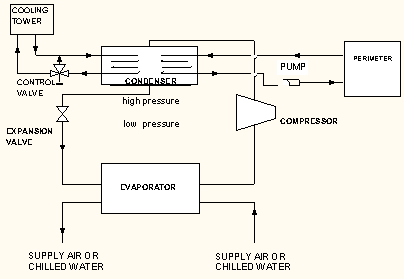
\includegraphics[width=0.9\textwidth, height=0.9\textheight, keepaspectratio=true]{media/image3175.png}
\caption{Diagram of Chiller:Electric with Heat Recovery \protect \label{fig:diagram-of-chiller-electric-with-heat}}
\end{figure}

The algorithm for the heat recovery portion of the chiller needs to be determined from relatively simple inputs to estimate the amount of the heat that is recovered and then send the rest of the heat to the cooling tower. For the chiller models associated with the object Chiller:Electric, air- or evaporatively-cooled condensers are allowed to be used with heat recovery and, when used, the condenser specific heat, mass flow rate, and temperatures shown below refer to outdoor air. A condenser air volume flow rate must be specified when using heat recovery with air- or evaporatively-cooled chillers.

The basic energy balance for the condenser section of a heat recovery chiller is

\begin{equation}
{\dot Q_{tot}} = {\dot Q_{Evap}} + {\dot Q_{Elec}} = {\dot Q_{Cond}} + {\dot Q_{HR}}
\end{equation}

In practice, if the entering temperature of the heat recovery hot fluid is too high, the chiller's internal controls will redirect refrigerant away from the heat recovery bundle.~ A user input is available for declaring the inlet high temperature limit, and if it is exceeded, the chiller will shut down heat recovery and request no flow and will not reject any condenser heat to that fluid.

The heat recovery condenser bundle is often physically smaller than the tower water condenser bundle and therefore may have limited heat transfer capacity.~ User input for the relative capacity of the heat recovery bundle, \({F_{HR,Cap}}\), is used to define a maximum rate of heat recovery heat transfer using

\begin{equation}
{\dot Q_{HR,Max}} = {F_{HR,Cap}}\left( {{{\dot Q}_{Evap,Ref}} + \frac{{{{\dot Q}_{Evap,Ref}}}}{{CO{P_{Ref}}}}} \right)
\end{equation}

This capacity factor is also used to autosize the heat recovery design fluid flow rate when it is set to autosize.~ The design heat recover flow rate is calculated by multiplying \({F_{HR,Cap}}\) by the condenser tower water design flow rate.~ If no capacity factor is input, it is assumed to be 1.0.

A heat recovery chiller may control the temperature of heat recovery fluid leaving the device by modulating the flow of refrigerant to the heat recovery condenser bundle.~ There are two different algorithms used depending on if the input has declared a leaving setpoint node.

If no control setpoint node was named, then the model developed by Liesen and Chillar (2004) is used to approximate the relative distribution of refrigerant flow and condenser heat transfer between the bundles.~ This model approximates the heat transfer situation by using average temperatures in and out of the condenser section.

\begin{equation}
{Q_{Tot}} = ({\dot m_{Heat{\mathop{\rm Re}\nolimits} c}}*{C_{p,Heat{\mathop{\rm Re}\nolimits} c}} + {\dot m_{Cond}}*{C_{p,Cond}})*({T_{AvgOut}} - {T_{AvgIn}})
\end{equation}

Then the inlet temperature is flow-weighted to determine lumped inlet and outlet conditions.

\begin{equation}
{T_{AvgIn}} = \frac{{({{\dot m}_{Heat{\mathop{\rm Re}\nolimits} c}}*{C_{p,Heat{\mathop{\rm Re}\nolimits} c}}*{T_{Heat{\mathop{\rm Re}\nolimits} cIn}} + {{\dot m}_{Cond}}*{C_{p,Cond}}*{T_{CondIn}})}}{{({{\dot m}_{Heat{\mathop{\rm Re}\nolimits} c}}*{C_{p,Heat{\mathop{\rm Re}\nolimits} c}} + {{\dot m}_{Cond}}*{C_{p,Cond}})}}
\end{equation}

\begin{equation}
{T_{AvgOut}} = \frac{{{Q_{Tot}}}}{{({{\dot m}_{Heat{\mathop{\rm Re}\nolimits} c}}*{C_{p,Heat{\mathop{\rm Re}\nolimits} c}} + {{\dot m}_{Cond}}*{C_{p,Cond}})}} + {T_{AvgIn}}
\end{equation}

The lumped outlet temperature is then used for an approximate method of determining the heat recovery rate

\begin{equation}
{\dot Q_{HR}} = {\dot m_{HR}}{c_p}_{HR}\left( {{T_{Avg,out}} - {T_{HR,in}}} \right)
\end{equation}

This rate is then limited by the physical size of the heat recovery bundle.

\begin{equation}
{\dot Q_{HR}} = Min\left( {{{\dot Q}_{HR}},{{\dot Q}_{HR,max}}} \right)
\end{equation}

If user input for the leaving temperature setpoint is available, then a second model is used to distribute refrigerant flow and condenser heat transfer between the bundles that attempts to meet the heat recovery load implied by the leaving setpoint.~ When setpoint control is used, the desired rate of heat recovery heat transfer is:

\begin{equation}
{\dot Q_{HR,Setpoint}} = {\dot m_{HR}}{c_p}_{HR}\left( {{T_{HR,set}} - {T_{HR,in}}} \right)
\end{equation}

\begin{equation}
{\dot Q_{HR,Setpoint}} = Max\left( {{{\dot Q}_{HR,Setpoint}},0.0} \right)
\end{equation}

Then the heat recovery rate is simply modeled as the lower of the three different heat flow rates:~ the desired capacity, the maximum capacity, and the current total heat rejection rate.

\begin{equation}
{\dot Q_{HR}} = Min\left( {{{\dot Q}_{HR,Setpoint}},{{\dot Q}_{HR,max}},{{\dot Q}_{Tot}}} \right)
\end{equation}

For both models, the condenser heat transfer rate is then

\begin{equation}
{\dot Q_{Cond}} = {\dot Q_{Tot}} - {\dot Q_{HR}}
\end{equation}

The outlet temperatures are then calculated using

\begin{equation}
  T_{HR,out} = T_{HR,in} + \frac{\dot{Q}_{HR}}{\dot{m}_{HR}C_{p,HR}}
\end{equation}

\begin{equation}
  T_{Cond,out} = T_{Cond,in} + \frac{\dot{Q}_{Cond}}{\dot{m}_{Cond}C_{p,Cond}}
\end{equation}

A heat recovery chiller may need to work harder because the refrigeration system faces a higher lift owing to an elevated effective temperature for heat rejection.~ With heat recovery, the condenser temperature used with the chiller's performance curves is determined using one of the following heat-flow-weighted methods. The first is used for the chiller model for the objects Chiller:Electric, and Chiller:Electric:EIR which use the condensing entering temperature for performance.

\begin{equation}
{T_{Cond,in,Avg}} = \frac{{\left( {{{\dot Q}_{HR}}{T_{HR,in}} + {{\dot Q}_{Cond}}{T_{Cond,in}}} \right)}}{{\left( {{{\dot Q}_{HR}} + {{\dot Q}_{Cond}}} \right)}}
\end{equation}

The second is used for the chiller model for the object Chiller:Electric:ReformulatedEIR which uses the leaving condenser fluid temperature.

\begin{equation}
{T_{Cond,out,Avg}} = \frac{{\left( {{{\dot Q}_{HR}}{T_{HR,out}} + {{\dot Q}_{Cond}}{T_{Cond,out}}} \right)}}{{\left( {{{\dot Q}_{HR}} + {{\dot Q}_{Cond}}} \right)}}
\end{equation}

Both of these are available as an output variable called Chiller Effective Heat Rejection Tempeature in \(^{\circ}\)C.

\subsubsection{Chiller Basin Heater}\label{chiller-basin-heater-2}

This chiller's basin heater (for evaporatively-cooled condenser type) operates in the same manner as the Engine driven chiller's basin heater. The calculations for the chiller basin heater are described in detail at the end of the engine driven chiller description (Ref. Engine Driven Chiller).

\textbf{Reference}

Liesen and Chillar. 2004. Variable Heat Recovery In Double Bundle Electric Chillers. SimBuild 2004, IBPSA-USA National Conference Boulder, CO, August 4-6, 2004.

\subsection{Electric Chiller Model Based on Fluid Temperature Differences}\label{electric-chiller-model-based-on-fluid-temperature-differences}

The centrifugal chiller model (object name Chiller:Electric) was originally developed for the BLAST program.~ The model is based on a `capacity ratio' curve, which is a quadratic equation that determines the Ratio of Available Capacity to Nominal Capacity. The defining equation is:

\begin{equation}
CapRatio = \frac{{Available Chiller Capacity}}{{Nominal Chiller Capacity}} = {A_1} + {A_2}\Delta {T_{chiller}} + {A_3}\Delta {T_{chiller}}^2
\end{equation}

where the Delta Temperature is defined as:

\begin{equation}
\Delta {T_{chiller}} = \frac{{{T_{cond, in}} - {T_{cond,in,design}}}}{{TempRiseRatio}} - \left( {{T_{evap,out}} - {T_{evap,out,design}}} \right)
\end{equation}

where the temperature rise coefficient is defined as the ratio of the required change in condenser water temperature to a given change in chilled water temperature, which maintains the capacity at the nominal value.~ If the chiller is a heat recovery chiller,then the condenser inlet temperature is adjusted to account for both fluid streams as described in the section above on heat recovery chillers. This is calculated as the following ratio:

\begin{equation}
TempRiseRatio = \frac{{{T_{cond, in,required}} - {T_{cond,in,rated}}}}{{{T_{evap, out,required}} - {T_{evap,out,rated}}}} - \left( {{T_{evap,out}} - {T_{evap,out,design}}} \right)
\end{equation}

where:

\emph{T\(_{cond,in,required}\)} is the required entering condenser air or water temperature to maintain rated capacity (\(^{\circ}\)C)

\emph{T\(_{cond,in,rated}\)} is the rated entering condenser air or water temperature at rated capacity (\(^{\circ}\)C)

\emph{T\(_{evap,out,required}\)} is the required leaving evaporator water outlet temperature to maintain rated capacity (\(^{\circ}\)C)

\emph{T\(_{evap,out,rated}\)} is the rated leaving evaporator water outlet temperature at rated capacity (\(^{\circ}\)C)

The Power Ratio Curve is a quadratic equation that determines the Ratio of Full Load to Power.~ The defining equation is:

\begin{equation}
PowerRatio = {B_1} + {B_2}PLR + {B_3}PL{R^2}
\end{equation}

where the part load ratio, PLR is defined as:

\begin{equation}
PLR = \frac{{chiller~cooling~load}}{{nominal~chiller~capacity}}
\end{equation}

The Load Ratio Curve is a quadratic equation that determines the Ratio of Actual Cooling Load to Full Cooling Load.~ The defining equation is:

\begin{equation}
LoadRatio = {C_1} + {C_2}CapRatio + {C_3}CapRati{o^2}
\end{equation}

The evaporator heat transfer rate and the power required by the chiller are then calculated as:

\begin{equation}
Qevap = AvailableChillerCap*PLR
\end{equation}

\begin{equation}
Power = PowerRatio*LoadRatio*\frac{{AvailableChillerCap}}{{RatedCOP}}
\end{equation}

\subsection{Electric Chiller Model Based on Condenser Entering Temperature}\label{electric-chiller-model-based-on-condenser-entering-temperature}

\subsubsection{Overview}\label{overview-2-003}

This model (object name Chiller:Electric:EIR) simulates the performance of an electric liquid chiller. The model is based on the compression chiller model (COMREF) in the DOE-2.1 building energy simulation program. The EnergyPlus model contains all of the features of the DOE-2.1 chiller model, plus additional abilities for modeling evaporatively-cooled condensers and heat recovery for water heating.

This model simulates the thermal performance of the chiller and the power consumption of the compressor(s). It also models the power consumption of condenser fans if modeling an air-cooled or evaporatively-cooled condenser. This model does not simulate the thermal performance or the power consumption of associated pumps or cooling towers. This auxiliary equipment must be modeled using other EnergyPlus models (e.g.~CoolingTower:SingleSpeed).

\subsubsection{Model Description}\label{model-description-2-003}

The chiller model uses user-supplied performance information at reference conditions along with three performance curves (curve objects) for cooling capacity and efficiency to determine chiller operation at off-reference conditions. The three performance curves are:

\begin{enumerate}
\item Cooling Capacity Function of Temperature Curve
\item Energy Input to Cooling Output Ratio Function of Temperature Curve
\item Energy Input to Cooling Output Ratio Function of Part Load Ratio Curve
\end{enumerate}

The cooling capacity function of temperature curve is a biquadratic performance curve with two independent variables: the leaving chilled water temperature and the entering condenser fluid temperature. The output of this curve is multiplied by the reference capacity to give the full-load cooling capacity at specific temperature operating conditions (i.e., at temperatures different from the reference temperatures). The curve should have a value of 1.0 at the reference temperatures and flow rates specified in the input data file by the user. The biquadratic curve should be valid for the range of water temperatures anticipated for the simulation. If the chiller is a heat recovery chiller,then the condenser inlet temperature is adjusted to account for both fluid streams as described in the section above on heat recovery chillers.

Note: The curve is evaluated at the leaving chilled water (=evaporator outlet) \emph{setpoint} temperature, not the \emph{actual} leaving chilled water temperature.

\begin{equation}
ChillerCapFTemp = a + b\left( {{T_{cw,ls}}} \right) + c{\left( {{T_{cw,ls}}} \right)^2} + d\left( {{T_{cond,e}}} \right) + e{\left( {{T_{cond,e}}} \right)^2} + f\left( {{T_{cw,ls}}} \right)\left( {{T_{cond,e}}} \right)
\end{equation}

where:

\emph{ChillerCapFTemp} is the cooling capacity factor, equal to 1 at reference conditions

\emph{T\(_{cw,ls}\)} is the leaving chilled water \emph{setpoint} temperature (\(^{\circ}\)C)

\emph{T\(_{cond,e}\)} is the entering condenser fluid temperature (\(^{\circ}\)C). For a water-cooled condenser this will be the water temperature returning from the condenser loop (e.g., leaving the cooling tower). For air- or evap-cooled condensers this will be the entering outdoor air dry-bulb or wet-bulb temperature, respectively.

\bigskip

The energy input to cooling output ratio function of temperature curve is a biquadratic performance curve that parameterizes the variation of the energy input to cooling output ratio (EIR) as a function of the leaving chilled water temperature and the entering condenser fluid temperature. The EIR is the inverse of the COP. The output of this curve is multiplied by the reference EIR (inverse of the reference COP) to give the full-load EIR at specific temperature operating conditions (i.e., at temperatures different from the reference temperatures). The curve should have a value of 1.0 at the reference temperatures and flow rates specified in the input data file by the user. The biquadratic curve should be valid for the range of water temperatures anticipated for the simulation.

\begin{equation}
ChillerEIRFTemp = a + b\left( {{T_{cw,l}}} \right) + c{\left( {{T_{cw,l}}} \right)^2} + d\left( {{T_{cond,e}}} \right) + e{\left( {{T_{cond,e}}} \right)^2} + f\left( {{T_{cw,l}}} \right)\left( {{T_{cond,e}}} \right)
\end{equation}

where:

\emph{ChillerEIRFTemp} is the energy input to cooling output factor, equal to 1 at reference conditions

\emph{T\(_{cw,l}\)} is the leaving chilled water temperature (\(^{\circ}\)C)

\emph{T\(_{cond,e}\)} is the entering condenser fluid temperature (\(^{\circ}\)C). For a water-cooled condenser this will be the water temperature returning from the condenser loop (e.g., leaving the cooling tower). For air- or evap-cooled condensers this will be the entering outdoor air dry-bulb or wet-bulb temperature, respectively. If the chiller is a heat recovery chiller,then the condenser inlet temperature is adjusted to account for both fluid streams as described in the section above on heat recovery chillers.

\bigskip

The energy input to cooling output ratio function of part-load ratio curve is a quadratic performance curve that parameterizes the variation of the chiller input power ratio as a function of the part-load ratio. The part-load ratio is the actual cooling load divided by the chiller's available cooling capacity. The output of this curve \textit{ChillerEIRFPLR} is multiplied by the reference EIR (inverse of the reference COP), chiller capacity as a function of temperature curve \textit{ChillerCapFTemp} and the Energy Input to Cooling Output Ratio Function of Temperature Curve \textit{ChillerEIRFTemp} to give the normalized power input at the specific temperature and part-load ratio at which the chiller is operating. Normalized power input is the ratio of chiller power input at a given operating condition to the chiller power input at reference condition. This curve should have a value of 1.0 when the part-load ratio equals 1.0. The quadratic curve should be valid for the range of part-load ratios anticipated for the simulation.

\begin{equation}
  \begin{array}{rl}
    ChillerEIRFPLR &= a + b\PB{PLR} + c\PB{PLR}^2\\
                   &= \frac{P_{chiller}}{{P_{ref}}\left( {ChillerCapFTemp} \right)\left( {ChillerEIRFTemp} \right)}
  \end{array}
\end{equation}

where:

\emph{ChillerEIRFPLR} = energy input to cooling output factor, equal to 1 at reference conditions

\emph{PLR} = part-load ratio = (cooling load) / (chiller's available cooling capacity)

\emph{P\(_{chiller}\) = chiller power at specific PLR}

\emph{P\(_{ref}\) = \({Q^\cdot_{ref}}\) /COP\(_{ref}\)}.

All three of the performance curves are accessed through EnergyPlus' built-in performance curve equation manager (curve:quadratic and curve:biquadratic). It is not imperative that the user utilize all coefficients in the performance curve equations if their performance equation has fewer terms (e.g., if the user's ChillerEIRFPLR performance curve is linear instead of quadratic, simply enter the values for a and b, and set coefficient c equal to zero). Performance curves for more than 160 chillers, including the default DOE-2.1E reciprocating and centrifugal chillers, are provided in the EnergyPlus Reference DataSets (Chillers.idf and AllDataSets.idf).

Note: Chiller:Electric:EIR objects and their associated performance curve objects are developed using performance information for a specific chiller and should normally be used together for an EnergyPlus simulation. Changing the object input values, or swapping performance curves between chillers, should be done with caution.

For any simulation time step, the chiller's available cooling capacity is calculated as follows:

\begin{equation}
{\dot{Q}_{avail}} = {\dot{Q}_{ref}}\left( {ChillerCapFTemp} \right)
\end{equation}

where:

\(\dot{Q}_{ref}\) is the chiller capacity at reference conditions (reference temperatures and flow rates defined by the user) (W)

\(\dot{Q}_{avail}\) is the available chiller capacity adjusted for current fluid temperatures (W).

The model then calculates the evaporator heat transfer rate required to bring the entering chilled water temperature down to the leaving chilled water setpoint temperature (established using a SetpointManager object and referenced in the PlantLoop object). If this calculated heat transfer rate is greater than the heat transfer rate being requested by the plant equipment operation scheme, then the evaporator heat transfer rate is reset to the requested cooling rate.

The evaporator heat transfer rate is then compared to the available capacity. If the available chiller capacity is sufficient to meet the evaporator heat transfer rate, the leaving chilled water temperature is set equal to the chilled water setpoint temperature. If the requested evaporator heat transfer rate is larger than the available capacity the chilled water leaving the evaporator is allowed to float upward. For this case, the exiting chilled water temperature is calculated based on the water temperature entering the evaporator, the available cooling capacity, and the evaporator mass flow rate as follows:

\begin{equation}
  T_{cw,l} = T_{cw,e} - \frac{\dot{Q}_{avail}}{\dot{m}_{evap}C_{p,evap}}
\end{equation}

where:

\emph{T\(_{cw,l}\)} is the water temperature leaving the evaporator (\(^{\circ}\)C)

\emph{T\(_{cw,e}\)} is the water temperature entering the evaporator (\(^{\circ}\)C)

\(\dot{m}_{evap}\) is the evaporator mass flow rate (kg/s)

\emph{C\(_{p,evap}\)} is the specific heat of water entering evaporator at \emph{T\(_{cw,e}\)} (J/kg-\(^{\circ}\)C).

The part-load ratio is then calculated as the ratio of the evaporator heat transfer rate to the available chiller capacity. The part-load ratio is not allowed to be greater than the maximum part-load ratio specified by the user or less than zero as follows:

\begin{equation}
  PLR = \max\PB{0.0,\min\PB{\frac{\dot{Q}_{evap}}{\dot{Q}_{avail}},PLR_{max}}}
\end{equation}

where:

\emph{PLR} is the part-load ratio

\({\dot{Q}_{evap}}\) is the load to be met by the chiller (W)

\emph{PLR\(_{max}\)} is the maximum part-load ratio (specified by the user in the input data file).

The model assumes that the cooling load is met through chiller unloading down to the minimum unloading ratio. False loading (e.g.~hot-gas bypass) is assumed to occur between the minimum unloading ratio and the minimum part load ratio yielding constant electrical power consumption under these conditions. Below the minimum part load ratio, the chiller cycles on and off to meet very small loads and the power consumption during the on cycle is the same as when the chiller is operating at the minimum part load ratio. When the chiller part load ratio is less than the minimum part load ratio, the on-off cycling ratio of the chiller is calculated as follows and is available as an output variable.

\begin{equation}
  ChillerCyclingRatio = \min\PB{\frac{PLR}{PLR_{min}},1.0}
\end{equation}

To properly account for chiller electric power consumption when PLR is less than the minimum unloading ratio, the PLR is reset to the greater of the PLR calculated above and the PLR at the minimum unloading ratio. The result is available as the output variable Chiller Part Load Ratio.

\begin{equation}
PLR = MAX(PLR,PL{R_{MinUnloadRatio}})
\end{equation}

This revised PLR accounts for the ``false loading'' (e.g., hot gas bypass) that is assumed to occur whenever the PLR (based on cooling load divided by available capacity) is less than the minimum unloading ratio specified. The amount of false loading on the chiller is calculated using this revised PLR and is reported as an output variable as follows:

\begin{equation}
{\dot{Q}_{falseloading}} = \left( {{\dot{Q}_{avail}}} \right)\left( {PLR} \right)\left( {ChillerCyclingRatio} \right) - {\dot{Q}_{evap}}
\end{equation}

The electrical power consumption for the chiller compressor(s) for any simulation time step is then calculated using the following equation:

\begin{equation}
{P_{chiller}} = \left( {{\dot{Q}_{avail}}} \right)\,\left( {\frac{1}{{CO{P_{ref}}}}} \right)\,\left( {ChillerEIRFTemp} \right)\left( {ChillerEIRFPLR} \right)\left( {ChillerCyclingRatio} \right)
\end{equation}

where:

\emph{P\(_{chiller}\)} is the chiller compressor power (W)

\emph{COP\(_{ref}\)} is the reference coefficient of performance (W/W).

Heat rejected by the chiller condenser includes the heat transferred in the evaporator plus a portion or all of the compressor electrical energy consumption. For electric chillers with hermetic compressors, all compressor energy consumption is rejected by the condenser (compressor motor efficiency = \emph{eff\(_{motor}\)} = 1.0). For chillers with semi-hermetic or open compressors, only a portion of the compressor energy use is rejected by the condenser. The heat transfer rate for the chiller condenser is calculated as follows:

\begin{equation}
{\dot{Q}_{cond}} = \left( {{P_{chiller}} * ef{f_{motor}}} \right) + {\dot{Q}_{evap}} + {\dot{Q}_{falseloading}}
\end{equation}

where:

\({\dot{Q}_{cond}}\) is the condenser heat transfer rate (W)

\(ef{f_{motor}}\) is the compressor motor efficiency = fraction of compressor electrical energy consumption rejected as condenser heat.

For water-cooled chillers, the water temperature leaving the condenser is then calculated as shown below.

\begin{equation} 
  T_{cond,l} = T_{cond,e} + \frac{\dot{Q}_{cond}}{\dot{m}_{cond}C_{p,cond}}
\end{equation}

where:

\emph{T\(_{cond,l}\)} is the water temperature leaving the condenser (\(^{\circ}\)C)

\emph{T\(_{cond,e}\)} is the water temperature entering the condenser (\(^{\circ}\)C)

\({\dot{m}_{cond}}\) is the mass flow rate through the condenser, kg/s

\({C_{p,cond}}\) is the specific heat of water entering the condenser at \emph{T\(_{cond,e}\)}, J/kg-(\(^{\circ}\)C).

For air- and evaporatively-cooled condensers, the exiting air temperature is not calculated and is set equal to the entering air or wet-bulb temperature, respectively.

The model then calculates the condenser fan energy for air- and evaporatively-cooled condensers. The amount of condenser fan energy is assumed to be proportional to the chiller cycling ratio and is calculated as follows:

\begin{equation}
{P_{cond}}\, = \,{\dot{Q}_{ref}}\,\left( {{P_{condfanratio}}} \right)\,\left( {ChillerCyclingRatio} \right)
\end{equation}

where:

\emph{P\(_{cond}\)} is the chiller condenser fan electric power (W)

\emph{P\(_{condfanratio}\)} is the condenser fan power ratio (W/W).

The final calculations determine the total heat transfer energy for the condenser and evaporator, as well as the total electric energy consumed by the chiller compressor motor(s) and condenser fan(s). The results are available as output variables.

\begin{equation}
{Q_{cond}} = {\dot{Q}_{cond}}*TimeStepSys*3600
\end{equation}

\begin{equation}
{Q_{evap}} = {\dot{Q}_{evap}}\,\,*\,\,TimeStepSys\,\,*\,\,3600
\end{equation}

\begin{equation}
{E_{chiller}} = {P_{chiller}}*\,\,TimeStepSys\,\,*\,\,3600
\end{equation}

\begin{equation}
{E_{cond}} = {P_{cond}}\,\, * \,\,TimeStepSys\,\,*\,\,3600
\end{equation}

where:

\emph{Q\(_{cond}\)} is the chiller condenser heat transfer energy (J)

\emph{Q\(_{evap}\)} is the chiller evaporator cooling energy (J)

\emph{E\(_{chiller}\)} is the chiller (compressor) electric energy (J)

\emph{E\(_{cond}\)} is the chiller condenser fan electric energy (J)

\emph{TimeStepSys} is the HVAC system simulation time step (hr)

\(3600\) is the conversion factor (sec/hr).

\subsubsection{Electric EIR Chiller with Heat Recovery Option}\label{electric-eir-chiller-with-heat-recovery-option}

Heat from the electric EIR chiller condenser may be recovered when a water-cooled condenser is selected for simulation. The heat recovery water flow rate is specified by the user along with the input and output nodes connected to the heat recovery loop. The algorithms are identical to those used for Chiller:Electric. Refer to the section entitled Chillers with Plant Heat Recovery for details.

\subsubsection{Standard Rating (Integrated Part Load Value)}\label{standard-rating-integrated-part-load-value}

For the Chiller:Electric:EIR and Chiller:Electric:ReformulatedEIR objects in EnergyPlus, the industry standard rating of Integrated Part Load Value (IPLV) is calculated according to ANSI/AHRI Standard 550/590 (2011). This standard rating is not direct input to the model and is calculated using user-entered information for these objects. These standard rating values are provided in the eplusout.eio output file (Ref. Output Details document) and also in the predefined tabular output reports (Output:Table:SummaryReports object, Equipment Summary).

\begin{callout}
Note: The standard ratings described in this section require that the EIR/Reformulated EIR chiller models be evaluated at specific operating conditions (e.g., specific evaporator outlet temperature (6.67\(^{\circ}\)C) and dry-bulb temperatures for air entering the air-cooled {[}outdoor{]} condenser). If the chiller~ performance curves can not be evaluated at the required test conditions, then the standard rating value will be determined at user specified curve limit and warning error message is provided. For example, if the curve object (Curve:Biquadratic) for Cooling Capacity Function of Temperature Curve has a minimum value of 21\(^{\circ}\)C for dry-bulb temperature entering the air-cooled condenser coil, the IPLV calculation requires that EER\(_{D}\) be calculated at 13\(^{\circ}\)C -- so, this would result in IPLV value calculated at 21\(^{\circ}\)C and reported in the output and a warning message in the eplusout.err file.
\end{callout}

The IPLV is a single number part-load performance figure of merit for Water-Chilling Packages. The IPLV equations and procedures described below are taken from Appendix D of ANSI/AHRI Std. 550/590, 2011 and provide a consistent method for calculating IPLV. These equations provide representative average part-load efficiency for a single chiller. ~For equipment covered by this standard, the \emph{IPLV} is calculated using the following formula:

\begin{equation}
IPLV = (0.01A) + (0.42B) + (0.45C) + (0.12D)
\end{equation}

where:

\(A\) is the \emph{EER} or \emph{COP} at 100\% capacity at AHRI standard rating conditions

\(B\) is the \emph{EER} or \emph{COP} at 75\% capacity and reduced ambient (see Table~\ref{table:standard-rating-integrated-part-load-value})

\(C\) is the \emph{EER} or \emph{COP} at 50\% capacity and reduced ambient (see Table~\ref{table:standard-rating-integrated-part-load-value})

\(D\) is the \emph{EER} or \emph{COP} at 25\% capacity and reduced ambient (see Table~\ref{table:standard-rating-integrated-part-load-value}).

The Coefficient of Performance (\emph{COP}) at the various load capacity points (100\%, 75\%, 50\%, and 25\% part-load ratios) are calculated using the procedure outlined below and applicable test conditions specified in Table~\ref{table:standard-rating-integrated-part-load-value}.

EER at desired reduced capacity (75\%, 50\%, and 25\%) is calculated as follows

\begin{equation}
COP = \frac{{\rm{1}}}{{EIR}}
\end{equation}

\begin{equation}
EIR = EnergyInputRatio = \left( {\frac{{{\rm{Power }}}}{{{\rm{PartLoadRatio * AvailChillerCap}}}}} \right)
\end{equation}

\begin{equation}
Power = \left( {\frac{{{\rm{AvailChillerCap}}}}{{CO{P_{reference}}}}} \right)(EIRTempModFa{c_{ReducedTemp}})(EIRPLRModFa{c_{ReducedPLR}})
\end{equation}

\begin{equation}
AvailChillerCap = Capacit{y_{reference}}(CAPTempModFa{c_{ReducedTemp}})
\end{equation}

where:

\(Capacit{y_{reference}}\) is the reference chiller capacity specified by the user (W)

\(CO{P_{reference}}\) is the reference coefficient of performance specified by the user (W/W)

\(EIRTempModFa{c_{ReducedTemp}}\) is the user-specified bi-quadratic curve for modifying EIR as a function of leaving chilled water temperature (6.7°C) and entering condenser temperature obtained from Table~\ref{table:standard-rating-integrated-part-load-value} for reduced capacities (dimensionless)

\(EIRPLRModFa{c_{ReducedPLR}}\) is the user-specified quadratic curve for modifying EIR as a function of part load ratio

\(CapTempModFa{c_{ReducedTemp}}\) is the capacity (W) of the chiller determined per the ANSI/AHRI Standard 550/590 reduced ambient test conditions as shown in Table~\ref{table:standard-rating-integrated-part-load-value}.

If the equipment cannot be unloaded to the desired reduced capacity (75\%, 50\%, and 25\%) i.e.~if the minimum unloading ratio of the chiller is greater than desired reduced capacity, then the model is run at the minimum unloading PLR of the equipment at the condenser entering conditions defined in Table~\ref{table:standard-rating-integrated-part-load-value} and the efficiency is adjusted for cyclic performance.

\begin{equation}
COP = \frac{{\rm{1}}}{{{C_D} \cdot EIRatMinPLR}}
\end{equation}

where:

\(EIRatMinPLR\) is the EIR of chiller at minimum unloading ratio

\({C_D}\) is the degradation coefficient to account for cycling of the compressor for capacity less than the minimum capacity.

The degradation coefficient \emph{C\(_{D}\)} for the desired reduced load points (75\%, 50\%, or 25\%) is determined using the following equation:

\begin{equation}
{C_D} = 1.13 - 0.13LF
\end{equation}

The load factor (\emph{LF}) for the desired reduced load points (75\%, 50\%, or 25\%) calculated from the following equation:

\begin{equation}
LF = \frac{{\left( {\frac{{\% Load}}{{100}}} \right) \cdot Full~load~unit~capacity}}{{Part~load~unit~capacity}}
\end{equation}

where:

\emph{\(\left( {\frac{{\% Load}}{{100}}} \right)\)} is the standard rating part load ratio (\emph{PLR}) points, 75\%, 50\%, 25\%

\(Full~load~unit~capacity\) is the full load heating capacity (W) of the air-source heat pump equipment determined from ANSI/AHRI Standard 550/590 and test conditions shown in Table~\ref{table:standard-rating-integrated-part-load-value} for 100\% load

\(Part~load~unit~capacity\) is the part load heating capacity (W) of the air-source heat pump units determined from ANSI/AHRI Standard 550/590 at the standard desired reduced ambient test conditions as shown in Table~\ref{table:standard-rating-integrated-part-load-value} and the minimum part load capacity of the unit.

\begin{equation}
Full~load~unit~capacity = {\dot Q_{total,Reference}}\left( {CapTempModFa{c_{Rated}}} \right)
\end{equation}

\begin{equation}
Part~load~unit~capacity = MinPLR \cdot {\dot Q_{total,Reference}}\left( {CapTempModFa{c_{ReducedTemp}}} \right)
\end{equation}

where:

\({\dot Q_{total,Reference}}\) is the reference capacity specified by the user (W)

\(CapTempModFa{c_{Rated}}\) is the user-specified bi-quadratic curve evaluated at full load (100\%) test conditions shown in Table~\ref{table:standard-rating-integrated-part-load-value} (dimensionless)

\(CapTempModFa{c_{ReducedTemp}}\) is the part load capacity (W) of the chiller determined from ANSI/AHRI Standard 550/590 at the standard desired reduced ambient test conditions as shown in Table~\ref{table:standard-rating-integrated-part-load-value}

\(MinPLR\) = Minimum PLR up to which chiller can be unloaded.

% table 51
\begin{longtable}[c]{p{1.2in}p{1.2in}p{1.2in}p{1.2in}p{1.2in}}
\caption{Standard Rating (Integrated Part Load Value) \label{table:standard-rating-integrated-part-load-value}} \tabularnewline
\toprule
 & \multicolumn{2}{c}{IPLV} & \multicolumn{2}{c}{NPLV} \tabularnewline
\midrule
\endfirsthead

\caption[]{Standard Rating (Integrated Part Load Value)} \tabularnewline
\toprule
 & \multicolumn{2}{c}{IPLV} & \multicolumn{2}{c}{NPLV} \tabularnewline
\midrule
\endhead

Evaporator (All types) & & & & \tabularnewline
100\% Load LWT & \(^{2}\)44.0\(^{\circ}\)F & 6.7\(^{\circ}\)C & \(^{2}\)Selected LWT & \(^{2}\)Selected LWT \tabularnewline
0\% Load LWT & \(^{2}\)44.0\(^{\circ}\)F & 6.7\(^{\circ}\)C & Same as 100\% load & Same as 100\% load \tabularnewline
Flow Rate (gpm) & \(^{3}\)2.4 gpm/ton & 0.043 L/s per kW & \(^{3}\)Selected ~~~~~~~~ gpm/ton & \(^{3}\)L/s per kW \tabularnewline
F.F.A & 0.0001 ~~~~~~~~~~~~~~~ h-ft\(^{2}\)-\(^{\circ}\)F/Btu & 0.000018 ~~~~~~~~ m\(^{2}\)-\(^{\circ}\)C/W & As Specified & As Specified \tabularnewline
\midrule
1 Condenser (Water  Cooled) & & & & \tabularnewline
100\% load EWT & 85.0\(^{\circ}\)F & 29.4\(^{\circ}\)C & \(^{2}\)Selected EWT & \(^{2}\)Selected EWT \tabularnewline
75\% load EWT & 75.0\(^{\circ}\)F & 23.9\(^{\circ}\)C & \(^{4}\) & \(^{4}\) \tabularnewline
50\% load EWT & 65.0\(^{\circ}\)F & 18.3\(^{\circ}\)C & \(^{4}\) & \(^{4}\) \tabularnewline
25\% load EWT & 65.0\(^{\circ}\)F & 18.3\(^{\circ}\)C & \(^{4}\) & \(^{4}\) \tabularnewline
0\% load EWT & 65.0\(^{\circ}\)F & 18.3\(^{\circ}\)C & 65.0\(^{\circ}\)F & 18.3\(^{\circ}\)C \tabularnewline
Flow rate (gpm) & \(^{3}\)3.0 gpm/ton & 0.054 L/s per kW & \(^{3}\)Selected ~~~~~~~~ gpm/ton & \(^{3}\)L/s per kW \tabularnewline
F.F.A. & 0.00025 ~~~~~~~~~~~~~~~ h-ft\(^{2}\)-\(^{\circ}\)F/Btu & 0.000044 ~~~~~~~~ m\(^{2}\)-\(^{\circ}\)C/W & As Specified & As Specified \tabularnewline
\midrule
\(^{1}\)Condenser (Air Cooled) & & & & \tabularnewline
100\% load EDB & 95.0\(^{\circ}\)F & 35.0\(^{\circ}\)C & \multicolumn{2}{l}{No Rating Requirements} \tabularnewline
75\% load EDB & 80.0\(^{\circ}\)F & 26.7\(^{\circ}\)C & & \tabularnewline
50\% load EDB & 65.0\(^{\circ}\)F & 18.3\(^{\circ}\)C & & \tabularnewline
25\% load EDB & 55.0\(^{\circ}\)F & 12.8\(^{\circ}\)C & & \tabularnewline
0\% load EDB & 55.0\(^{\circ}\)F & 12.8\(^{\circ}\)C & & \tabularnewline
F.F.A. & 0.0 h-ft\(^{2}\)-\(^{\circ}\)F/Btu & 0.0 m\(^{2}\)-\(^{\circ}\)C/W & & \tabularnewline
\midrule
\(^{1}\)Condenser (Evaporatively Cooled) & & & & \tabularnewline
100\% load EWB & 75.0\(^{\circ}\)F & 23.9\(^{\circ}\)C & \multicolumn{2}{l}{No Rating Requirements} \tabularnewline
0\% load EWB & 50.0\(^{\circ}\)F & 10.0\(^{\circ}\)C & & \tabularnewline
F.F.A. & 0.0 h-ft\(^{2}\)-\(^{\circ}\)F/Btu & 0.0 m\(^{2}\)-\(^{\circ}\)C/W & & \tabularnewline
\midrule
Air-Cooled Without  Condenser & & & & \tabularnewline
100\% load SDT & 125.0\(^{\circ}\)F & 51.7\(^{\circ}\)C & \multicolumn{2}{l}{No Rating Requirements} \tabularnewline
0\% load SDT & 55.0\(^{\circ}\)F & 12.8\(^{\circ}\)C & & \tabularnewline
\midrule
Water and Evaporatively Cooled Without Condenser & & & & \tabularnewline
100\% load SDT & 105.0\(^{\circ}\)F & 40.6\(^{\circ}\)C & \multicolumn{2}{l}{No Rating Requirements} \tabularnewline
0\% load SDT & 65.0\(^{\circ}\)F & 18.3\(^{\circ}\)C & & \tabularnewline
\bottomrule
\multicolumn{5}{l}{\(^{1}\) If the unit Manufacturer’s recommended minimum temperatures are greater than those} \tabularnewline
\multicolumn{5}{l}{specified in Table 3, then those may be used in lieu of the specified temperatures.} \tabularnewline
\multicolumn{5}{l}{\(^{2}\) Correction for Fouling Factor Allowance} \tabularnewline
\multicolumn{5}{l}{\(^{3}\) The flow rates are to be held constant at full load values for all part-load conditions.} \tabularnewline
\multicolumn{5}{l}{\(^{4}\) For part-load entering condenser water temperatures, the temperature should vary} \tabularnewline
\multicolumn{5}{l}{linearly from the selected} \tabularnewline
\multicolumn{5}{l}{EWT at 100\% load to 65.0 oF at 50\% loads, and fixed at 65.0°F for 50\% to 0\% loads.} \tabularnewline
\multicolumn{5}{l}{SDT - saturated discharge temperature} \tabularnewline
\multicolumn{5}{l}{LWT - leaving water (liquid) temperature} \tabularnewline
\multicolumn{5}{l}{EWT - entering water (liquid) temperature} \tabularnewline
\multicolumn{5}{l}{EDB - entering air dry-bulb temperature} \tabularnewline
\multicolumn{5}{l}{EWB - entering air wet-bulb temperature} \tabularnewline
\multicolumn{5}{l}{F.F.A. - Fouling Factor Allowance} \tabularnewline
\multicolumn{5}{c}{\scriptsize Source: Table 3, Page 10, ANSI/AHRI Standard 550/590-2011}
\end{longtable}

\subsection{Electric Chiller Model Based on Condenser Leaving Temperature}\label{electric-chiller-model-based-on-condenser-leaving-temperature}

\subsubsection{Overview}\label{overview-3-002}

This model (object name Chiller:Electric:ReformulatedEIR) simulates the thermal performance of an electric liquid chiller and the power consumption of its compressor(s). The model, developed by Hydeman et al. (2002) as part of the CoolTools™ project sponsored by Pacific Gas and Electric Company (PG\&E), is an empirical model similar to EnergyPlus' Chiller:Electric:EIR model. The model uses performance information at reference conditions along with three curve fits for cooling capacity and efficiency to determine chiller operation at off-reference conditions. The model has the same capabilities as the Chiller:Electric:EIR model, but can potentially provide significant accuracy improvement over the Chiller:Electric:EIR model for chillers with variable-speed compressor motor drives and/or variable condenser water flow applications.

Chiller performance curves can be generated by fitting manufacturer's catalog data or measured data. Performance curves developed primarily from manufacturer's performance data are provided in the EnergyPlus Reference DataSets (Chillers.idf and AllDataSets.idf). This chiller model can be used to predict the performance of various chiller types (e.g., reciprocating, screw, scroll, and centrifugal) with water-cooled condensers. The model does not simulate the thermal performance or the power consumption of associated pumps or cooling towers. This auxiliary equipment must be modeled using other EnergyPlus models (e.g.~CoolingTower:SingleSpeed).

The main difference between this model and the Chiller:Electric:EIR model is the condenser fluid temperature used in the associated performance curves: the Chiller:Electric:ReformulatedEIR model uses the LEAVING condenser water temperature while the Chiller:Electric:EIR model uses the ENTERING condenser water temperature. In addition, the Energy Input to Cooling Output Function of Part Load Ratio curve for this reformulated EIR chiller model includes the condenser leaving water temperature as an independent variable in addition to part-load ratio. Since the leaving condenser water temperature is a function of load, chiller performance, and condenser entering water temperature, EnergyPlus must iterate to converge on a solution for each simulation time step.

\subsubsection{Model Description}\label{model-description-3-002}

The chiller model uses user-supplied performance information at reference conditions along with three performance curves (curve objects) for cooling capacity and efficiency to determine chiller operation at off-reference conditions. The three performance curves are:

1)~~~~Cooling Capacity Function of Temperature Curve

2)~~~~Energy Input to Cooling Output Ratio Function of Temperature Curve

3)~~~~Energy Input to Cooling Output Ratio Function of Part Load Ratio Curve

The cooling capacity function of temperature curve is a biquadratic performance curve with two independent variables: the leaving chilled water temperature and the leaving condenser water temperature. The output of this curve is multiplied by the reference capacity to give the full-load cooling capacity at specific temperature operating conditions (i.e., at temperatures different from the reference temperatures). The curve should have a value of 1.0 at the reference temperatures and flow rates specified in the input data file by the user. The biquadratic curve should be valid for the range of water temperatures anticipated for the simulation (otherwise the program issues warning messages).

\begin{equation}
ChillerCapFTemp = a + b({T_{cw,l}}) + c{({T_{cw,l}})^2} + d({T_{cond,l}}) + e{({T_{cond,l}})^2} + f({T_{cw,l}})({T_{cond,l}})
\end{equation}

where:

\emph{ChillerCapFTemp} is the cooling capacity factor, equal to 1 at reference conditions

\emph{T\(_{cw,l}\)} is the leaving chilled water temperature (\(^{\circ}\)C)

\emph{T\(_{cond,l}\)} is the leaving condenser water temperature (\(^{\circ}\)C). This will be the water temperature entering the condenser loop (e.g., entering the cooling tower). If the chiller is a heat recovery chiller,then the condenser leaving temperature is adjusted to account for both fluid streams as described in the section above on heat recovery chillers.

The energy input to cooling output ratio function of temperature curve is a biquadratic performance curve that parameterizes the variation of the energy input to cooling output ratio (EIR) as a function of the leaving chilled water temperature and the leaving condenser water temperature. The EIR is the inverse of the COP. The output of this curve is multiplied by the reference EIR (inverse of the reference COP) to give the full-load EIR at specific temperature operating conditions (i.e., at temperatures different from the reference temperatures). The curve should have a value of 1.0 at the reference temperatures and flow rates specified in the input data file by the user. The biquadratic curve should be valid for the range of water temperatures anticipated for the simulation (otherwise the program issues warning messages).

\begin{equation}
ChillerEIRFTemp = a + b({T_{cw,l}}) + c{({T_{cw,l}})^2} + d({T_{cond,l}}) + e{({T_{cond,l}})^2} + f({T_{cw,l}})({T_{cond,l}})
\end{equation}

where:

\emph{ChillerEIRFTemp} is the energy input to cooling output factor, equal to 1 at reference conditions

\emph{T\(_{cw,l}\)} is the leaving chilled water temperature (\(^{\circ}\)C)

\emph{T\(_{cond,l}\)} is the leaving condenser water temperature (\(^{\circ}\)C). This will be the water temperature entering the condenser loop (e.g., entering the cooling tower). If the chiller is a heat recovery chiller,then the condenser leaving temperature is adjusted to account for both fluid streams as described in the section above on heat recovery chillers.

The energy input to cooling output ratio function of part-load ratio curve parameterizes the variation of the energy input ratio (EIR). The output of this curve is multiplied by the reference EIR (inverse of the reference COP) and the Energy Input to Cooling Output Ratio Function of Temperature Curve to give the EIR at the specific temperatures and part-load ratio at which the chiller is operating. This curve should have a value of 1.0 at the reference leaving condenser water temperature with part-load ratio equal to 1.0. It is recommended that this performance curve be developed using both full- and part-load performance data. The bicubic curve should be valid for the range of condenser water temperatures and part-load ratios anticipated for the simulation (otherwise the program issues warning messages). Either of the following two types of curves can be used.

The first type is a bicubic performance curve that parameterizes the variation of the chiller input power ratio as a function of the leaving condenser water temperature and the part-load ratio. The part-load ratio is the actual cooling load divided by the chiller's available cooling capacity.

\begin{equation}
ChillerEIRFPLR = a + b({T_{cond,l}}) + c{({T_{cond,l}})^2} + d(PLR) + e{(PLR)^2} + f({T_{cond,l}})(PLR) + g{(PLR)^3}
\end{equation}

\begin{equation}
  ChillerEIRFPLR = \frac{P_{chiller}}{P_{ref}}\left( {ChillerCapFTemp} \right)\left( {ChillerEIRFTemp} \right)
\end{equation}

where:

\emph{ChillerEIRFPLR} is the energy input to cooling output factor, equal to 1 at the reference leaving condenser water temperature and PLR = 1.0

\emph{T\(_{cond,l}\)} is the leaving condenser water temperature (\(^{\circ}\)C). This will be the water temperature entering the condenser loop (e.g., entering the cooling tower). If the chiller is a heat recovery chiller,then the condenser leaving temperature is adjusted to account for both fluid streams as described in the section above on heat recovery chillers.

\emph{PLR} is the part load ratio = (cooling load) / (chiller's available cooling capacity)

\emph{P\(_{chiller}\) is the chiller power at specific PLR}

\emph{P\(_{ref}\) = \({\dot{Q}_{ref}}\) /COP\(_{ref}\)}.

Note: Although a bicubic curve requires 10 coefficients (ref. Curve:Bicubic), coefficients 7, 9 and 10 are typically not used in the performance curve described here and should be entered as 0 unless sufficient performance data and regression accuracy exist to justify the use of these terms of the bicubic curve.

The second type is a Chiller Part Load Custom Curve that parameterizes the variation of EIR as a function of the normalized dT, normalized Tdev and the PLR.

\begin{equation}
\begin{split}
ChillerEIRFPLR = a + b(dT^*) + c(dT^*)^2 + d \cdot PLR + e \cdot PLR^2 + f \cdot (dT^*) \cdot PLR + g \cdot (dT^*)^3 \\
+ h \cdot PLR^3 + i \cdot (dT^*)^2 \cdot PLR + j \cdot (dT^*) \cdot PLR^2 + k \cdot (dT^*)^2 \cdot PLR^2 + l \cdot (T_{dev}^*) \cdot PLR^3
\end{split}
\end{equation}

\begin{equation}
dT^* = dT / dT_{ref}
\end{equation}

\begin{equation}
T_{dev}^* = T_{dev} / dT_{ref}
\end{equation}

where:

\(dT\) is the delta of temperature across the leaving condenser water temperature and leaving evaporator water temperature of a chiller (lift)

\(dT^*\) is the normalized fractional lift

\(dT_{ref}\) is the lift under the reference condition

PLR is the part load ratio

\(T_{dev}\) is the deviation of leaving chilled water temperature from the reference condition

\(T_{dev}^*\) is the normalized Tdev term.

All of these performance curves are accessed through EnergyPlus' built-in performance curve equation manager (curve:biquadratic, curve:bicubic, and Curve:ChillerPartLoadWithLift). Note that the above three performance curves use the leaving condenser water temperature as an independent variable, instead of the entering condenser water temperature used in the performance curves for the Chiller:Electric:EIR model. Since the leaving condenser water temperature is calculated based on the condenser heat transfer rate, which is a function of the load to be met by the chiller, chiller compressor power, and the false loading (detailed calculations are given below), iterative calculations are required to determine the actual (converged) leaving condenser water temperature. The program uses the leaving condenser water temperature from the previous iteration to calculate values for each of the three performance curves described above. After obtaining the condenser heat transfer rate, the leaving condenser water temperature is recalculated. When the difference between the leaving condenser water temperature calculated on successive iterations is less than 0.0001\(^{\circ}\)C, the solution is assumed to have converged. Warning messages are issued if the calculated solution for leaving condenser water temperature and/or part-load ratio falls outside the valid range specified for the chiller's performance curves. If these warnings are issued, the user may choose to extend the range for the performance curves (only if a small extension is required since model extrapolation may produce significant errors) or a different chiller and associated performance curves with extended performance range can be located and used for the simulation.

Note: Chiller:Electric:ReformulatedEIR objects and their associated performance curve objects are developed using performance information for a specific chiller and should almost always be used together for an EnergyPlus simulation. Changing the object input values, or swapping performance curves between chillers, should be done with extreme caution. For example, if the user wishes to model a chiller size that is different from the reference capacity, it is highly recommended that the reference flow rates be scaled proportionately to the change in reference capacity. Although this model can provide more accurate prediction than the Chiller:Electric:EIR model, it requires more performance data to develop the associated performance curves (at least 12 points from full-load performance and 7 points from part-load performance).

Although performance curve data sets for 160 chillers are provided in the EnergyPlus Reference DataSets (Chillers.idf and AllDataSets.idf), they may not meet the requirements for specific applications. One can develop performance curves from performance data using two available techniques (Hydeman and Gillespie 2002). The first technique is called the Least-squares Linear Regression method and is used when sufficient performance data exist to employ standard least-square linear regression techniques. The second technique is called Reference Curve Method and is used when insufficient performance data exist to apply linear regression techniques. A detailed description of both techniques can be found in the reference mentioned above.

For any simulation time step, the chiller's available cooling capacity is calculated as follows:

\begin{equation}
{\dot{Q}_{avail}}\,\, = \,\,{\dot{Q}_{ref}}\left( {ChillerCapFTemp} \right)
\end{equation}

where

\({\dot{Q}_{ref}}\) is the chiller capacity at reference conditions (reference temperatures and flow rates defined by the user) (W)

\({\dot{Q}_{avail}}\) is the available chiller capacity adjusted for current water temperatures (W).

The model then calculates the evaporator heat transfer rate required to bring the entering chilled water temperature down to the leaving chilled water setpoint temperature (established using a SetpointManager object and referenced in the PlantLoop object). If this calculated heat transfer rate is greater than the heat transfer rate being requested by the plant equipment operation scheme, then the evaporator heat transfer rate is reset to the requested cooling rate.

The evaporator heat transfer rate is then compared to the available capacity. If the available chiller capacity is sufficient to meet the evaporator heat transfer rate, the leaving chilled water temperature is set equal to the chilled water setpoint temperature. If the requested evaporator heat transfer rate is larger than the available capacity the chilled water leaving the evaporator is allowed to float upward. For this case, the exiting chilled water temperature is calculated based on the water temperature entering the evaporator, the available cooling capacity, and the evaporator mass flow rate as follows:

\begin{equation}
  T_{cw,l}  =  T_{cw,e} - \frac{\dot{Q}_{avail}}{\dot{m}_{evap}C_{p,evap}}
\end{equation}

where:

\emph{T\(_{cw,l}\)} is the water temperature leaving the evaporator (\(^{\circ}\)C)

\emph{T\(_{cw,e}\)} is the water temperature entering the evaporator (\(^{\circ}\)C)

\({\dot{m}_{evap}}\) is the evaporator mass flow rate (kg/s)

\emph{C\(_{p,evap}\)} is the specific heat of water entering evaporator at \emph{T\(_{cw,e}\)} (J/kg-\(^{\circ}\)C).

The part-load ratio is then calculated as the ratio of the evaporator heat transfer rate to the available chiller capacity. The part-load ratio is not allowed to be greater than the maximum part-load ratio specified by the user or less than zero as follows:

\begin{equation}
  PLR = \max\PB{0.0,\min\PB{\frac{\dot{Q}_{evap}}{\dot{Q}_{avail}},PLR_{max}}}
\end{equation}

where:

\emph{PLR} is the part-load ratio

\({\dot{Q}_{evap}}\) is the load to be met by the chiller (W)

\emph{PLR\(_{max}\)} is the maximum part-load ratio (specified by the user in the input data file).

Note that the maximum part-load ratio (PLR\(_{max}\), specified in the Chiller:Electric:ReformulatedEIR object) used in the equation should be less than or equal to the maximum part-load ratio specified in the ``Energy Input to Cooling Output Ratio Function of Part-Load Ratio'' performance curve object.

The model assumes that the cooling load is met through chiller unloading down to the minimum unloading ratio. False loading (e.g.~hot-gas bypass) is assumed to occur between the minimum unloading ratio and the minimum part-load ratio yielding constant electrical power consumption under these conditions. Below the minimum part-load ratio, the chiller cycles on/off to meet very small loads and the power consumption during the on cycle is the same as when the chiller is operating at the minimum part load ratio. When the chiller part-load ratio is less than the minimum part-load ratio, the on-off cycling ratio of the chiller is calculated as follows and is available as an output variable.

\begin{equation}
  ChillerCyclingRatio = \min \PB{ \frac{PLR}{PLR_{min}}, 1.0 }
\end{equation}

To properly account for chiller electric power consumption when PLR is less than the minimum unloading ratio, the PLR is reset to the greater of the PLR calculated above and the PLR at the minimum unloading ratio. The result is available as the output variable Chiller Part Load Ratio.

\begin{equation}
PLR = MAX(PLR,PL{R_{MinUnloadRatio}})
\end{equation}

This revised PLR accounts for the ``false loading'' (e.g., hot-gas bypass) that is assumed to occur whenever the PLR (based on cooling load divided by available capacity) is less than the minimum unloading ratio specified. The amount of false loading on the chiller is calculated using this revised PLR and is reported as an output variable as follows:

\begin{equation}
{\dot{Q}_{falseloading}} = \left( {{{\mathop Q\limits^ \bullet  }_{avail}}} \right)\left( {PLR} \right)\left( {ChillerCyclingRatio} \right) - {\dot{Q}_{evap}}
\end{equation}

The electrical power consumption for the chiller compressor(s) for any simulation time step is then calculated using the following equation:

\begin{equation}
{P_{chiller}}\, = \,\,\left( {{{\mathop Q\limits^ \bullet }_{avail}}\,} \right)\,\left( {\frac{1}{{CO{P_{ref}}}}} \right)\,\left( {ChillerEIRFTemp} \right)\left( {ChillerEIRFPLR} \right)\left( {ChillerCyclingRatio} \right)
\end{equation}

where:

\emph{P\(_{chiller}\)} is the chiller compressor power (W)

\emph{COP\(_{ref}\)} is the reference coefficient of performance (W/W).

Heat rejected by the chiller condenser includes the heat transferred in the evaporator plus a portion or all of the compressor electrical energy consumption. For electric chillers with hermetic compressors, all compressor energy consumption is rejected by the condenser (compressor motor efficiency = \emph{eff\(_{motor}\)} = 1.0). For chillers with semi-hermetic or open compressors, only a portion of the compressor energy use is rejected by the condenser. The heat transfer rate for the chiller condenser is calculated as follows:

\begin{equation}
{\dot{Q}_{cond}} = \left( {{P_{chiller}} * ef{f_{motor}}} \right) + {\dot{Q}_{evap}} + {\dot{Q}_{falseloading}}
\end{equation}

where:

\({\dot{Q}_{cond}}\) is the condenser heat transfer rate (W)

\(ef{f_{motor}}\) is the compressor motor efficiency = fraction of compressor electrical energy consumption rejected as condenser heat.

The above curve values are calculated based on the leaving condenser water temperature found through iteration. After obtaining the condenser heat transfer rate, the final leaving condenser water temperature is then calculated as:

\begin{equation}
  T_{cond,l} = T_{cond,e} + \frac{\dot{Q}_{cond}}{\dot{m}_{cond} C_{p,cond}}
\end{equation}

where:

\emph{T\(_{cond,l}\)} is the water temperature leaving the condenser (\(^{\circ}\)C)

\emph{T\(_{cond,e}\)} is the water temperature entering the condenser (\(^{\circ}\)C)

\({\dot{m}_{cond}}\) is the mass flow rate through the condenser (kg/s)

\({C_{p,cond}}\) is the specific heat of water entering the condenser at \emph{T\(_{cond,e}\)} (J/kg-\(^{\circ}\)C)

The final calculations determine the total heat transfer energy for the condenser and evaporator, as well as the total electric energy consumed by the chiller compressor motor(s) and condenser fan(s). The results are available as output variables.

\begin{equation}
{Q_{cond}} = {\dot{Q}_{cond}}*TimeStepSys*3600
\end{equation}

\begin{equation}
{Q_{evap}} = {\dot{Q}_{evap}}\,\,*\,\,TimeStepSys\,\,*\,\,3600
\end{equation}

\begin{equation}
{E_{chiller}} = {P_{chiller}}*\,\,TimeStepSys\,\,*\,\,3600
\end{equation}

\begin{equation}
{E_{cond}} = {P_{cond}}\,\, * \,\,TimeStepSys\,\,*\,\,3600
\end{equation}

where

\emph{Q\(_{cond}\)} is the chiller condenser heat transfer energy (J)

\emph{Q\(_{evap}\)} is the chiller evaporator cooling energy (J)

\emph{E\(_{chiller}\)} is the chiller (compressor) electric energy (J)

\emph{E\(_{cond}\)} is the chiller condenser fan electric energy (J)

\emph{TimeStepSys} is the HVAC system simulation time step (hr)

\(3600\) is a conversion factor (sec/hr).

\subsubsection{Electric Reformulated EIR Chiller with Heat Recovery Option}\label{electric-reformulated-eir-chiller-with-heat-recovery-option}

Heat from the electric reformulated EIR chiller condenser may be recovered. The heat recovery water flow rate is specified by the user along with the input and output nodes connected to the heat recovery loop. The algorithms are identical to those used for Chiller:Electric and Chiller:Electric:EIR. Refer to the section entitled Chillers with Plant Heat Recovery for details.

\subsubsection{Standard Rating (Integrated Part Load Value)}\label{standard-rating-integrated-part-load-value-1}

Integrated Part Laod Value (IPLV) calculations for Reformulated EIR chiller are similar to what are described above for EIR chillers. The only difference with Reformulated EIR chiller is that it calls an iterative subroutine (SolveRegulaFalsi) to obtain a condenser water outlet temperature which corresponds to condenser inlet temperature at reduced capacity conditions as outlined in Table~\ref{table:standard-rating-integrated-part-load-value} above. SolveRegulaFalsi is a general utility routine for finding the zero of a function. In this case it finds the condenser inlet temperature that will zero the residual function -- the difference between calculated condenser inlet temperature and desired condenser inlet temperature per ANSI/AHRI 550/590, 2011 (Table~\ref{table:standard-rating-integrated-part-load-value} above) divided by desired condenser inlet temperature.

\subsubsection{References}\label{references-1-003}

Hydeman, M., N. Webb, P. Sreedharan, and S. Blanc. 2002. Development and Testing of a Reformulated Regression-Based Electric Chiller Model. ASHRAE Transactions HI-02-18-2.

Hydeman, M. and K.L. Gillespie. 2002. Tools and Techniques to Calibrate Electric Chiller Component Models. ASHRAE Transactions AC-02-9-1.

Hydeman, M., K. Gillespie, and R. Kammerud. 1997. PG\&E's CoolTools project: A toolkit to improve evaluation and operation of chilled water plants. Presented at the Cool\$ense National Forum on Integrated Chilled Water Retrofits, Sep. 1997. Berkeley California: Lawrence Berkeley National Laboratory.

\subsection{Engine Driven Chiller}\label{engine-driven-chiller}

The engine driven chiller (Object name: Chiller:EngineDriven) is the empirical model from the Building Loads and System Thermodynamics (BLAST) program. Fitting catalog data to a third order polynomial equations generates the chiller performance curves.~ Three sets of coefficients are required to model the open centrifugal chiller as discussed in the section, titled, `Electric Chiller Based on Fluid Temperature Differences'. Additional curve fits are required to model the engine.~ Because the model inherently involves the lower heating value of the fuel, a reference temperature is also involved in the calculations, which manufacturers present at 25\(^{\circ}\)C.

The engine model was also developed for the BLAST program. It was adapted for use in EnergyPlus. This model is used for both the engine driven generator and the engine driven chiller.~ It uses the following set of equations all of which are quadratic fits to the PLR (Part Load Ratio) of the generator.~ The coefficients must be derived from manufacturers data.

\begin{equation}
\frac{{chiller\,\,cooling\,\,load}}{{fuel\,\,energy\,\,input}} = \frac{{chiller\,\,cooling\,\,load}}{{\left( {{{\dot m}_{fuel}}\left\{ {kg/s} \right\} \cdot LHV\left\{ {J/kg} \right\}} \right)}} = {a_1} + {a_2}PLR + {a_3}PL{R^2}
\end{equation}

The exhaust gas temp and flow rate are used if a stack heat exchanger is used to recover waste heat from the exhaust.~ This temperature is the inlet temperature to the heat exchanger which is modeled in a UA-effectiveness form:

\begin{equation}
\frac{{Total\,Exhaust\,heat}}{{fuel\,energy\,input}} = \frac{{Total\,\,Exhaust\,\,heat}}{{\left( {{{\dot m}_{fuel}}\left\{ {kg/s} \right\} \cdot LHV\left\{ {J/kg} \right\}} \right)}} = {d_1} + {d_2}PLR + {d_3}PL{R^2}
\end{equation}

\begin{equation}
\frac{{Exhaust\,\,Gas\,\,Temp\,\,\left\{ K \right\}}}{{fuel\,\,energy\,\,input}} = \frac{{Exhaust\,\,Gas\,\,Temp\,\,\left\{ K \right\}}}{{\left( {{{\dot m}_{fuel}}\left\{ {kg/s} \right\} \cdot LHV\left\{ {J/kg} \right\}} \right)}} = {e_1} + {e_2}PLR + {e_3}PL{R^2}
\end{equation}

The exhaust flow rate is then calculated as:

\begin{equation}
{\dot m_{exhaust}} = \frac{{Total\,\,Exhaust\,\,heat}}{{C{p_{exhaust}} \cdot \left( {{T_{exhaust}} - {T_{reference}}} \right)}}
\end{equation}

where T\(_{reference}\) is the reference temperature for the fuel lower heating value, and is given as 25\(^{\circ}\)C in manufacturer's data, and

\begin{equation}
{T_{stack}} = {T_{DesignMinExhaust}} + {\frac{{\left( {{T_{exhaust}} - {T_{DesignMinExhaust}}} \right)}}{{{\rm{exp}}\left( {\frac{{{\rm{UA}}}}{{{{{\rm{\dot m}}}_{{\rm{exhaust}}}}C{p_{exhaust}}}}} \right)}}^2}
\end{equation}

Finally, heat recovered from the lube oil and the water jacket are accounted for as follows:

\begin{equation}
\frac{{Recoverable\,\,jacket\,\,heat}}{{fuel\,\,energy\,\,input}} = \frac{{Recoverable\,\,jacket\,\,heat}}{{\left( {{{\dot m}_{fuel}}\left\{ {kg/s} \right\} \cdot LHV\left\{ {J/kg} \right\}} \right)}} = {b_1} + {b_2}PLR + {b_3}PL{R^2}
\end{equation}

\begin{equation}
\frac{{Recoverable\,\,lube\,\,oil\,\,heat}}{{fuel\,\,energy\,\,input}} = \frac{{Recoverable\,\,lube\,\,oil\,\,heat}}{{\left( {{{\dot m}_{fuel}}\left\{ {kg/s} \right\} \cdot LHV\left\{ {J/kg} \right\}} \right)}} = {c_1} + {c_2}PLR + {c_3}PL{R^2}
\end{equation}

\subsubsection{Chiller Basin Heater}\label{chiller-basin-heater-3}

Calculations are also made to estimate the electric power input to the basin heater for chillers with evaporatively-cooled condensers. The chillers which calculate basin heater power are Chiller:Electric:EIR, Chiller:Electric, Chiller:ConstantCOP, Chiller:EngineDriven and Chiller:CombustionTurbine.A schedule may be used to disable the basin heater during regular maintenance periods or other time periods (e.g., during summer). If a schedule is not provided, the basin heater is assumed to be available the entire simulation time period. The basin heater operates when it is scheduled on, the outdoor air dry-bulb temperature is below the basin heater setpoint temperature, and the chiller is not active (i.e., chiller is not operating for the simulation time step --- for example, when there is no cooling load to be met by the chiller, \emph{or if there is no water flow through the chiller due to a chiller or pump availability schedule, etc.}). The user is required to enter a basin heater capacity (watts per degree Kelvin) and a heater setpoint temperature (\(^{\circ}\)C) if they want to model basin heater electric power.

Here is sample of pseudo-code for the chiller basin heater model:

\(P_{heater,basin}\) = 0.0

IF (ChillerIsOFF) THEN

~~IF (Schedule\(_{heater,basin}\) is Defined) THEN

~~~~IF (CAP\(_{heater,basin}\) > 0 AND Schedule\(_{heater,basin}\) = ON) THEN

~~~~~~P\(_{heater,basin}\) = MAX(0.0,CAP\(_{heater,basin}\)*(T\(_{setpoint,basin}\)-T\(_{db,outdoor}\)))

~~~~ENDIF

~~ELSE

~~~~IF (CAP\(_{heater,basin} > 0)\) THEN

~~~~~~P\(_{heater,basin}\) = MAX(0.0,CAP\(_{heater,basin}\)*(T\(_{setpoint,basin}\)-T\(_{db,outdoor}\)))

~~~~ENDIF

~~ENDIF

ENDIF

\begin{equation}
{E_{heater,basin}} = \left( {{P_{heater,basin}}} \right)\left( {TimeStepSys} \right)3600
\end{equation}

where:

\({P_{heater,basin}}\) is the chiller basin heater electric power (W)

\({E_{heater,basin}}\) is the chiller basin heater electric consumption (J)

\emph{T\(_{setpoint,basin}\)} is the basin heater setpoint temperature, user input (\(^{\circ}\)C)

\emph{T\(_{db,outdoor}\)} is the outdoor air dry-bulb temperature (\(^{\circ}\)C)

\emph{CAP\(_{heater,basin}\)} is the basin heater capacity, user input (W/K)

\emph{Schedule\(_{heater,basin}\)} is the basin heater schedule, user input (schedule value \textgreater{} 0 means ON)

\emph{ChillerIsOFF} is the logical variable denoting that the chiller is not operating for the current simulation time step (e.g.,~ there is no cooling load to be met by the chiller, or if there is no water flow through the chiller due to a chiller or pump availability schedule, etc.). 
